\documentclass[11pt]{report}
\usepackage[german]{babel}
\usepackage[a4paper,top=2cm,bottom=2cm,left=3cm,right=3cm,marginparwidth=1.75cm]{geometry}
% Bildunterschriften 
\usepackage{caption}
\captionsetup{font=footnotesize} % Schriftgröße
\captionsetup{justification=centering} % Zentrierte Darstellung
\usepackage{float} % Bildplatzierung
\usepackage{graphicx}

\usepackage{enumitem} % Paket für Anpassung von Listen
\usepackage[bottom]{footmisc} % Fußnoten am Ende der Seite platzieren
\usepackage{amsmath}



\usepackage{pdfpages} % Includieren von PDF Dokumenten

% Linkdarstellung
\usepackage{hyperref}
\hypersetup{
    colorlinks=true,    % Links farbig hervorheben
    linkcolor=blue,     % Farbe interne Links
    urlcolor=blue,      % Farbe URLs
}

% Tabellenformatierung
\usepackage{booktabs} % Für schönere Linien
\usepackage{array}    % Für Spaltenanpassungen
\usepackage{multirow} % Für mehrzeilige Zellen
\usepackage{makecell} % Für Zellumbrüche

% Code Ausschnitte
\usepackage{listings}
\usepackage{xcolor}
\usepackage{soul}
\definecolor{codegreen}{rgb}{0,0.6,0}
\definecolor{codegray}{rgb}{0.5,0.5,0.5}
\definecolor{codepurple}{rgb}{0.58,0,0.82}
\definecolor{backcolour}{rgb}{0.70,0.70,0.70}

\lstset{language=C,keywordstyle={\bfseries \color{blue}}}

\lstdefinestyle{C_DTCO}{
    backgroundcolor=\color{backcolour},   
    commentstyle=\color{codegreen},
    keywordstyle=\color{codepurple},
    numberstyle=\tiny\color{codegray},
    stringstyle=\color{orange},
	frame=leftline|topline|bottomline|rightline,
	frameround=tttt,
    basicstyle=\ttfamily\footnotesize,
    breakatwhitespace=false,         
    breaklines=true,                 
    captionpos=b,                    
    keepspaces=true,                 
    numbers=left,                    
    numbersep=4pt,                  
    showspaces=false,                
    showstringspaces=false,
    showtabs=false,                  
    tabsize=1
}
\lstset{style=C_DTCO}

% Zeilenabstand
\usepackage[onehalfspacing]{setspace}

% Schriftart 
\usepackage[scaled]{helvet}
\usepackage[T1]{fontenc}
\renewcommand\familydefault{\sfdefault}

\title{Erzeugung eines 3D Pythagoras-Baums mit parallelen Technologien\\
        \large{Endbericht aus dem Fach Parallel Computing unter der Leitung von Marko Fehrenbach\\
                HTWG Konstanz | Wintersemester 2025 / 2026}
}

\author{Patrick Denz, Sofie Birkle, Tomke Velten}

\begin{document}
\pagenumbering{gobble}
\renewcommand{\figurename}{Abb.} % Abbildungsbeschriftung
%\documentclass[11pt]{report}
%\usepackage[german]{babel}
%\usepackage[a4paper,top=2cm,bottom=2cm,left=3cm,right=3cm,marginparwidth=1.75cm]{geometry}
%\usepackage{graphicx}
% Schrift
%\usepackage[scaled]{helvet}
%\usepackage[T1]{fontenc}
%\renewcommand\familydefault{\sfdefault}


%\begin{document}
\begin{titlepage}
	\centering
	{\scshape\LARGE HTWG Konstanz | Wintersemester 2025 / 2026 \par}
	\vspace{1cm}
	{\scshape\Large Endbericht aus dem Fach Parallel Computing \\
        unter Leitung von Marko Fehrenbach\par}
    \vspace{1.5cm}
    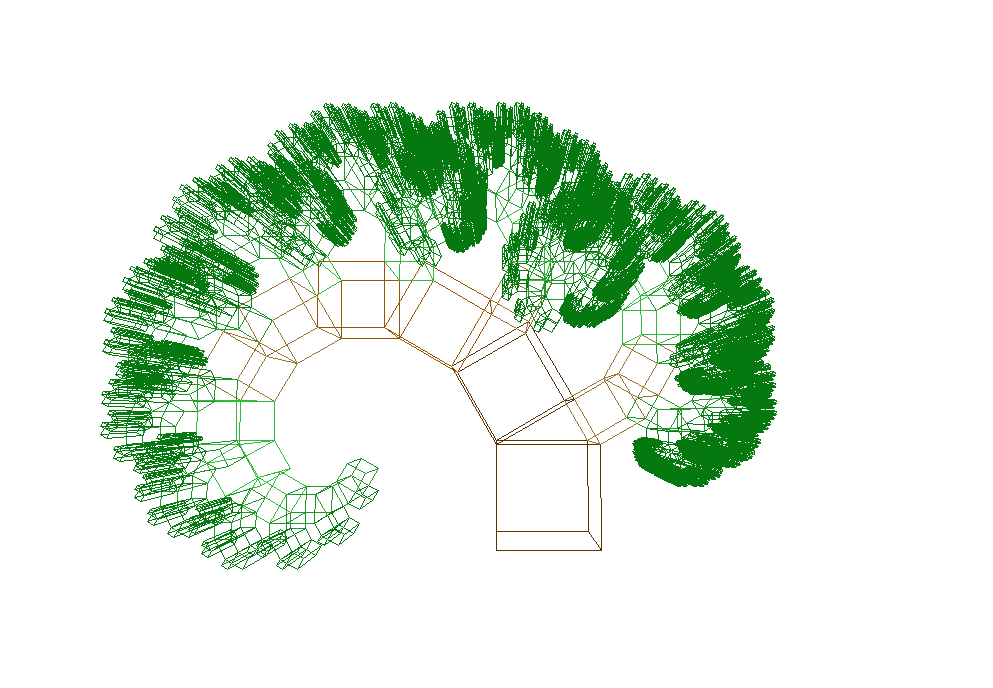
\includegraphics[width=0.95\linewidth]{./pictures/Deckblatt.PNG}\par\vspace{1cm}
	\vspace{1.5cm}
	{\huge Erzeugung eines 3D Pythagoras-Baums \\
        mit parallelen Technologien \par}
	\vspace{2cm}
	{\Large\itshape 
	Patrick Denz \textsc{(307728)} \\
    Sofie Birkle \textsc{(307550)} \\
    Tomke Velten \textsc{(307553)}\par}
	\vfill

% Bottom of the page
	{\large \today\par}
\end{titlepage}
%\end{document}

\centering
\section*{Abstract}
Pythagoras-Bäume sind Fraktale, deren Struktur sich aus einer wiederholten Anwendung derselben Operation auf eine Menge von Körpern ergibt. 
Ziel dieser Arbeit war die Erzeugung eines dreidimensionalen Pythagoras-Baums (Quader statt Quadrate) und die anschließende Parallelisierung der Berechnung mit 
unterschiedlichen Technologien. Ausgangspunkt war eine serielle Implementierung, die wir zunächst rekursiv und anschließend — zur besseren Parallelisierbarkeit
— iterativ (ebenenweise) umgesetzt haben. Für die korrekte Platzierung der Quader im 3D-Raum war dabei eine Verwendung von Transformationsmatrizen notwendig. \\

Darauf aufbauend parallelisierten wir datenparallel: OpenMP auf der CPU und OpenCL auf der GPU (bzw. auf PoCL/CPU, abhängig vom System). Neben der eigentlichen 
Generierung floss auch die Aufbereitung für einen einfachen SDL-basierten Wireframe-Renderer in die Gesamtlaufzeit ein. \\

Die Laufzeitmessungen auf mehreren Geräten zeigen, dass Parallelisierung bei kleinen Baumtiefen zunächst Overhead verursacht, bei größeren Tiefen jedoch deutliche 
Beschleunigungen ermöglicht (z. B. OpenMP bis ca. 93\% Zeitersparnis, OpenCL je nach Tiefe bis ca. 87\%). Limitiert wird die maximal erreichbare Baumtiefe primär durch 
den quadratisch wachsenden Speicherbedarf der Quaderdaten.

\raggedright
\tableofcontents
\newpage

\pagenumbering{arabic}
\setcounter{secnumdepth}{2} % Setzt die Tiefe der Nummerierung
\renewcommand\thesection{\arabic{section}} % Nummerierung der Hauptkapitel
\renewcommand\thesubsection{\arabic{section}.\arabic{subsection}} % Nummerierung der Unterkapitel

\setcounter{section}{-1} % Nummerierung bei 0 starten
\section{Vorwissen}
\vspace{-0.5cm}
\begin{minipage}{0.66\linewidth}
    Pythagoras-Bäume gehören zu den Fraktalen. Im zweidimensionalen Raum setzt sich ein Pythagoras-Baum aus 
    Quadraten zusammen, auf die jeweils ein rechtwinkliges Dreieck aufgesetzt werden, auf dessen Kanten
    wiederum Quadrate platziert werden.
    Sie tragen ihren Namen, da sich die Seitenlängen neuer Quadrate mittels dem Satz des Pythagoras 
    $a^2 + b^2 = c^2$ aus den Kantenlängen des aufgesetzten Dreiecks berechnen lassen.
\end{minipage}
\hfill
\begin{minipage}{0.3\linewidth}
    \centering
    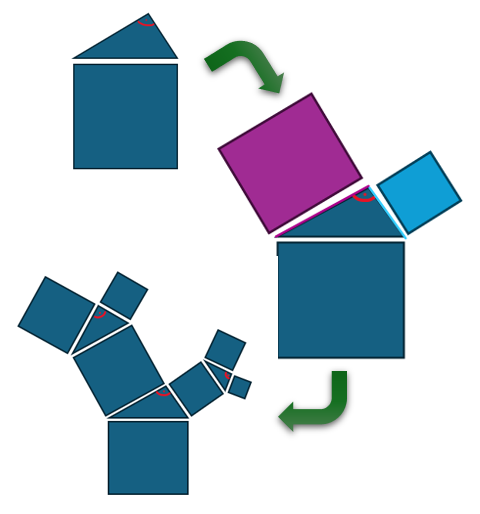
\includegraphics[width=\linewidth]{./pictures/Erzeugung-Pythagorasbaum.PNG}
    \captionof{figure}{Erzeugung eines Pythagoras-Baums}
    \label{fig:Erzeugung Baum}
\end{minipage}

\vspace{-0.5cm}
\subsection*{Mathematische Grundlagen}
\vspace{-0.25cm}
\subsubsection*{Kartesisches Koordinatensystem} \label{Koordinatensystem}
\vspace{-0.25cm}
\begin{minipage}{0.25\linewidth}
    \centering
    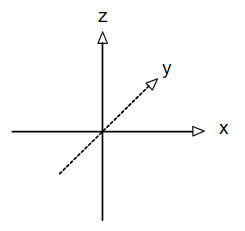
\includegraphics[width=0.8\linewidth]{./pictures/Koordinatensystem.PNG}
    \captionof{figure}{Achsenbeschriftung Koordinatensystem}
    \label{fig:koordinatensystem}
\end{minipage}
\hfill
\begin{minipage}{0.74\linewidth}
    Wir arbeiten mit einem dreidimensionalen Koordinatensystem, bei welchem die x-Achse bei frontaler 
    Betrachtung von links nach rechts verläuft, die y-Achse die Tiefe des Raums abbildet und die z-Achse 
    von unten nach oben verläuft.
\end{minipage}

\vspace{-0.25cm}
\subsubsection*{Bezeichner der Körper}\label{Koerper}
\vspace{-0.25cm}
\begin{minipage}{0.25\linewidth} % Würfel
    \centering
    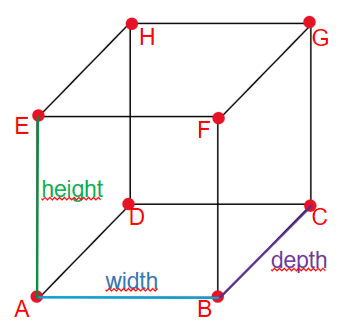
\includegraphics[width=\linewidth]{./pictures/Würfel.PNG}
    \captionof{figure}{Beschriftung Quader}
    \label{fig:wuerfel}
\end{minipage}
\hfill
\begin{minipage}{0.74\linewidth}
    Würfel / Quader\\
    Unsere Würfel und Quader sind definiert über die Ecken ABCD, welche das untere Quadrat bilden, und 
    die Ecken EFGH, welche das parallel darüberliegende Quadrat bilden.\\
    Darüber hinaus bestimmen die Seitenlängen width (entlang der x-Achse), depth (entlang der y-Achse) 
    und height (entlang der z-Achse) die Größe des Körpers.
\end{minipage}

\vspace{0.25cm} 
\noindent
\begin{minipage}{0.25\linewidth} % Dreieck
    \centering
    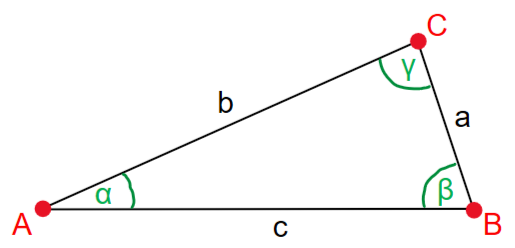
\includegraphics[width=\linewidth]{./pictures/Dreieck.PNG}
    \captionof{figure}{Beschriftung Dreieck}
    \label{fig:dreieck}
\end{minipage}
\hfill
\begin{minipage}{0.74\linewidth}
    Dreieck \\
    Dreiecke, die in unserem Programm für Dreiecksberechnungen wie den Sinussatz zum Einsatz kommen,
    folgen der in der Grafik dargestellten Beschriftung. Dabei ist $\gamma$ immer der rechte Winkel.
\end{minipage}

\subsubsection*{Betrag eines Vektors}\label{Vektorbetrag}
%\vspace{-0.25cm}
\[
\| \mathbf{v} \| = \sqrt{a^2 + b^2 + c^2}
\]

%\vspace{-0.25cm}
\subsubsection*{Sinussatz}\label{Sinussatz}
%\vspace{-0.25cm}\\
\[
\frac{a}{\sin(\alpha)} = \frac{b}{\sin(\beta)} = \frac{c}{\sin(\gamma)} \quad \Rightarrow \quad a = \frac{c}{\sin(\gamma)} \cdot \sin(\alpha),
\quad b = \frac{c}{\sin(\gamma)} \cdot \sin(\beta)
\]

\newpage
\section{Hardware und Rendering}
\subsection{Verwendete Hardware}\label{Hardware}
\begin{table}[h]
    \centering
\begin{tabular}{@{}lccc@{}}
    \toprule
    \textbf{Produkt}         & \textbf{ThinkPad P15 Gen 2}                       & \textbf{ThinkPad P14s Gen 1}           & \textbf{ASUS ZenBook 13}            \\
    \midrule
    \textbf{Prozessor}       & \makecell{Intel Core \\ i7-11850H}          & \makecell{AMD Ryzen 7 \\ PRO 4750U}    & \makecell{AMD Ryzen 7 \\ 5800 U}  
    \vspace{2mm} \\ % Abstand zwischen Sektionen
    \textbf{Taktung (in GHz)}&                                             &                                        &                                     \\ 
    minimale Frequenz:       & 2.5                                         & 1.7                                    & 1.9                                 \\ 
    Boost (ein Kern):        & 4.8                                         & 4.1                                    & 4.4                                 \\ 
    Boost (alle Kerne):      & (keine Angabe)                              & 3.1                                    & 3.4                       
    \vspace{3mm} \\ % Abstand zwischen Sektionen 
    \textbf{Parallelität}    &                                             &                                        &                                     \\
    Kerne                    & 8                                           & 8                                      & 8                                   \\
    Threads                  & 16                                          & 16                                     & 16 
    \vspace{3mm} \\ % Abstand zwischen Sektionen
    \textbf{RAM}             & 32 GB                                       & 24 GiB                                 & 16 GB                               \\ 
    Taktung:                 & 3200 MHz                                    & 3200 MHz                               & 3200 MHz                   
    \vspace{3mm}  \\ % Abstand zwischen Sektionen
    \textbf{Grafikkarte}     & \makecell{Nvidia RTX \\ A3000}              & \makecell{AMD Radeon \\ RX Vega 7}     & \makecell{AMD Radeon \\ RX Vega 8}  \\ 
    Größe:                   & 6 GB                                        & 2 GB                                   & 497 MB                     
    \vspace{3mm} \\ % Abstand zwischen Sektionen
    \textbf{Betriebssystem}  & Windows 10                                  & \makecell{Debian 13 \\ Kernel 6.12.63} & Windows 10                          \\ 
    \bottomrule
\end{tabular}
    \caption{Überblick der Gerätespezifikationen verwendeter Laptops}
\end{table}
\noindent
Während der Prozessor-Boost mit einem Kern für die Single-Thread-Performance relevant ist, ist der Boost mit mehreren Kernen 
für die Multi-Thread-Performance von Bedeutung.
\vspace{0.25cm}\\
\noindent
\textit{Anmerkung:} Auf dem Thinkpad P14s Gen 1 wurde OpenCL nicht nativ auf der Grafikkarte, sondern über PoCL\footnote{PoCL = Portable Computing Language --- 
u.a. für x86-Architektur geeignete Implementierung von OpenCL} auf der CPU ausgeführt. Grund dafür waren Kooperationsprobleme zwischen der integrierten 
AMD-Grafikkarte und den Linux-Treibern, die zu Systemabstürzen führten. Da dieses Problem ausschließlich auf dem Thinkpad P14s Gen 1 unter Linux auftrat und nicht
bei Nvidia unter Linux oder ähnlichen AMD-Grafikchips unter Windows, deutet dies auf ein Treiberproblem hin, nicht auf ein Problem mit unserem Programm.

\subsection{Crossplatform mit Linux und Windows}
Das Projekt selbst ist lauffähig unter Windows und Linux, sofern \lstinline{nvidia-opencl-dev} (o.ä. für die jeweilig verbaute Hardware) 
und \lstinline{libsdl2-dev} installiert sind. \\
Im Makefile werden die Bibliotheken wie folgt verwendet: \lstinline{LFLAGS = -lSDL2 -lSDL2main -lOpenCL} 
Für die Verwendung von OpenMP wird zusätzlich \lstinline{-fopenmp} bei den CXXFLAGS benötigt --- das Makefile des Linux-Projekts 
selbst stammt aus einem Plugin für die Projektgenerierung für C++.  
Da die Abgabe unter Windows mit Visual Studio 2022 erfolgen soll, haben wir den src-Ordner vom Visual Studio Projekt ins 
Linux-Projektverzeichnis verlinkt. \\
Eine Herausforderung während der Entwicklung für beide Plattformen war vor allem die Zeitmessung. Unter Linux wurde bei 
paralleler Ausführung anfangs die Zeit für alle Threads aufsummiert, was dann quasi der Zeit entsprach, die die serielle Version
benötigte. Unter Windows hingegen wurde die Zeit korrekt gemessen, allerdings fehlten hier die Funktionen, die zum Messen der 
Zeit unter Linux nötig waren.\\
Unsere Lösung war, die jeweilige Zeitmessung in einem Präprozessor-Block zu kapseln, sodass jede Plattform ihre eigene
Implementierung verwenden kann. 

\subsection{Renderer}
Ein Pythagorasbaum definiert sich durch sein Aussehen. Dementsprechend benötigten wir zur Vollendung unseres Projekts eine Möglichkeit,
unsere Ergebnisse visuell aufzubereiten. Da das Rendern von Grafiken kein wesentlicher Bestandteil der Lehrveranstaltung war, ließen wir uns
bei der Entwicklung eines Renderers durch Chat-GPT 5 unterstützen. \\
Unser Renderer verwendet zur Darstellunug der Daten die SDL-Bibliothek\footnote{SDL = Simple DirectMedia Layer; freie Multimedia-Bibliothek mit 
Unterstützung vieler Plattformen}.\\
\noindent
Die Punkte werden dort mittels einer Projektionsmatrix auf die Bildfläche übertragen. Die so entstehenden Bildpunkte 
werden anschließend mit der Information über die Verbindung untereinander (Kanten, engl. `Edges`) im dreidimensionalen 
Raum zu einer Wireframe-Grafik\footnote{Wireframe = Grafik, welche ausschließlich aus Kanten/Ecken besteht und keine 
Flächen beinhaltet} verarbeitet, da jede Verbindung im 3D-Raum direkt auf die 2D-Bildfläche übertragen werden kann. 
So entsteht eine 2D-Projektion, welche auf dem Bildschirm angezeigt wird. Die Kamera kann mit Hilfe von WASD 
nach links, rechts, oben und unten bewegt werden, wobei die Kamera immer auf einen Fixpunkt im Koordinatensystem
gerichtet bleibt.\\
Eine Redundanzprüfung, welche verhindern würde, dass übereinanderliegende und dadurch nicht sichtbare Punkte und 
Linien gerendert werden, haben wir --- obwohl sie die Effizienz des Renderers maßgeblich steigern könnte --- nicht 
implementiert, um uns auf die tatsächlichen Anforderungen des Kurses zu fokussieren. Um ein besseres visuelles 
Erlebnis zu ermöglichen, haben wir die tatsächlich aufeinanderliegenden Kanten mit der Funktion 
\texttt{removeRedundantEdges()} entfernt. 

% - mit Hilfe von KI erstellt
% - erstellt mit SDL (Simple Direct Media Layer) eine Wireframe-Grafik (nur Kanten/Ecken, keine Flächen)
% - verarbeitet Punkte und Informationen über Verbindung selbiger (Edges) im dreidimensionalen Raum zu einer Projektion in 2D 
% - auch doppelte Punkte / Linien werden ohne Prüfung der Sichtbarkeit verarbeitet -> keine Effizienzsteigerung durch Redundanzprüfung

% Einbindung ins Projekt? 

 % DONE

\newpage
\section{Sequentielle Realisierung}
Unser erster Schritt zu einem parallel berechneten Pythagoras-Baum war die serielle Umsetzung des Algorithmus, welche
uns bereits aus Programmiertechnik 2 bei Prof.~Bittel bekannt war. 

\vspace{-0.25cm}
\subsubsection*{Klassen}
\vspace{-0.25cm}
Um eine möglichst übersichtliche Projektstruktur zu erhalten, entschieden wir uns für eine Implementierung, bei der die einzelnen 
Bestandteile unseres Baums (Punkte, Quader, Dreiecke) als Klassen realisiert wurden.
Dabei definierten wir unser dreidimensionales \hyperref[Koordinatensystem]{Koordinatensystem} und einigten uns auf eine einheitliche
Benennungen der Ecken und Kanten unserer \hyperref[Koerper]{Körper}.

\vspace{-0.25cm}
\subsubsection*{Verschiebung der Objekte im Raum}
\vspace{-0.25cm}
    Die größte Herausforderung in der sequentiellen Umsetzung des Pythagoras-Baums bestand darin, die verschiedenen Komponenten korrekt 
    zu platzieren. Anders als im zweidimensionalen Raum kann der Punkt C des Dreiecks, welches auf der vorderen oberen Kante des Quaders 
    aufgesetzt wird, im Dreidimensionalen nicht einfach berechnet werden. \\
\begin{minipage}{0.3\linewidth}
    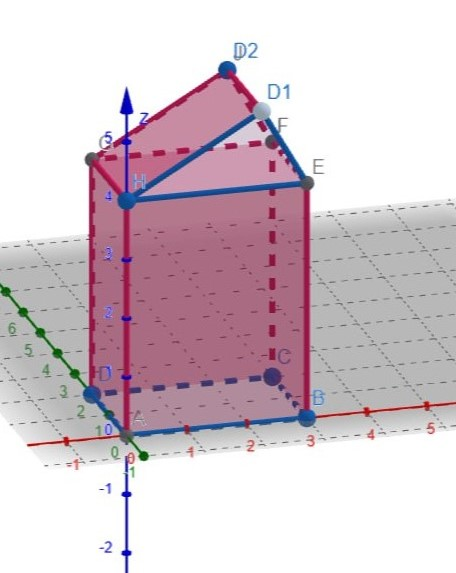
\includegraphics[width=\linewidth]{./pictures/Dreiecksberechnung_Geogebra.jpg}
    %\caption{Zu bestimmender Punkt - Geogebra}
\end{minipage}
\hfill
\begin{minipage}{0.68\linewidth}
    Unser erster Ansatz war das Umstrukturieren unserer im Zweidimensionalen funktionalen Methode zu einer im dreidimensionalen wirksamen 
    Funktion. Nach einiger Zeit stellte sich jedoch heraus, dass dies programmatisch und auch mathematisch in dieser Form nicht möglich ist.
\end{minipage}

\vspace{0.5cm}
\noindent
In Folge dessen entschieden wir uns für eine Lösung mit Transformationsmatrizen. Während wir die Seitenlänge eines neuen
Quaders weiterhin über trigonometrische Berechnungen bestimmten, wurde nun jeder neue Quader mit Ecke A im Koordinatenursprung (0|0|0) 
erzeugt. Anschließend wurde jeder Punkt einzeln mit Hilfe einer Rotationsmatrix an seine neue Position gedreht und um einen 
Vektor an die richtige Stelle im Koordinatensystem verschoben.

\noindent
\begin{figure}[h!]
    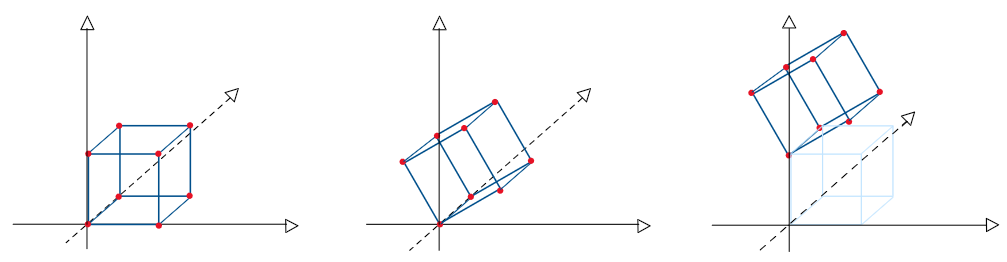
\includegraphics[width=\linewidth]{./pictures/Wuerfeltransformation.PNG}
    \caption{Transformation eines Quaders}
\end{figure}

% ----------------------------------- Rekursion ---------------------------------------
% ----------------------------------------------------------------------------------
\subsection{Rekursion}
\vspace{-0.25cm}
\begin{minipage}{0.59\linewidth}
    Der einfachste Weg zur Erzeugung eines Pythagoras-Baums, welcher uns bereits aus Programmiertechnik 2 bekannt war,
    ist eine rekursive Funktion. Diese ist so strukturiert, dass zu Beginn geprüft wird, ob die Abbruchbedingung erfüllt 
    ist. Falls ja, wird die Rekursion beendet. Anderenfalls wird die Seitenlänge des neuen Quaders berechnet. Anschließend
    ruft die Funktion sich mit ebendieser Länge selbst wieder auf.\\
    Diesem Ansatz entsprechend haben wir die Funktion \texttt{buildTree()} implementiert, bei welcher eine vorab festgelegte
    minimale Seitenlänge als Abbruchbedingung zum Einsatz kam.     
\end{minipage}
\hfill 
\begin{minipage}{0.39\linewidth}
    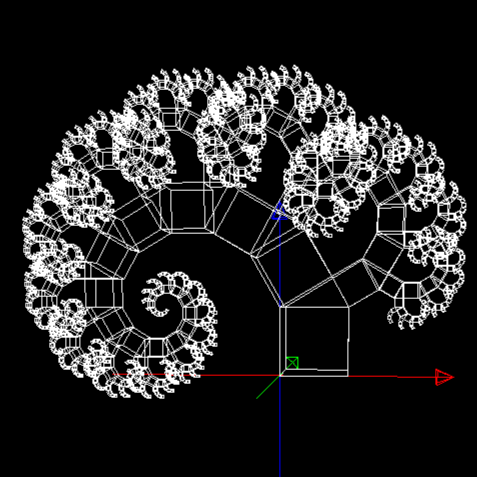
\includegraphics[width=\linewidth]{./pictures/seriell-fixed_0.1.PNG}
    \captionof{figure}{Pythagoras-Baum. \\Minimale Seitenlänge: 0.1, Winkel $\alpha$: 30°}
    \label{fig:BaumStatisch}
\end{minipage}
% Code von Branch parallel Commit-ID 016811b - sequentiell finished
\vspace{0.25cm}
\begin{lstlisting}[caption=Ausschnitt der rekursiven buildTree() Funktion]
 void buildTree(Cuboid cuboid, Renderer &renderer, double oldAngle) {
    if (siteLength < 0.05) { return; } // exit condition
    // Definition of render object
    RenderObject cube; 
    // ... add verts and edges of given cuboid to cube ...
    renderer.addRenderObject(cube);

    // Computation of next Cuboids
    double newAngle = oldAngle - 30;
    std::vector<double> newSidelength = getNewSidelength(points[3], points[2], 30);

    // create righthanded new Cuboid
    Cuboid newCuboid_b = Cuboid(getNextCuboid(newSidelength[1], newAngle, points[4].toStdVector()));
    std::vector<Point> cuboid_bPoints = newCuboid_b.getPoints();

    // create lefthanded new Cuboid
    Cuboid newCuboid_a = Cuboid(getNextCuboid(newSidelength[0], newAngle + 90, cuboid_bPoints[1].toStdVector()));

    // Recursion
    buildTree(newCuboid_b, renderer, newAngle);
    buildTree(newCuboid_a, renderer, newAngle + 90);
 }
\end{lstlisting}

% ----------------------------------- Iterativ ---------------------------------------
% ------------------------------------------------------------------------------------
\vspace{-0.5cm}
\subsection{Iterative Lösung}\label{iterativ}
\vspace{-0.25cm}
Da rekursive Funktionen, besonders solche, die mit einer Tail-Rekursion\footnote{Tail-Rekursion = Spezielle Form der Rekursion, 
bei der der rekursive Aufruf die letzte Aktion einer Funktion ist}
arbeiten, nicht effizient parallelisierbar sind, mussten wir unsere \texttt{buildTree()} Funktion im nächsten Schritt in eine iterative
Funktion umformen. Eine ebenenweise Erzeugung der Quader ermöglicht später das Verteilen der Berechnungen auf mehrere CPU-Kerne 
oder GPU-Threads.\\
Die neue Funktion \texttt{generateSerialIterative()} nimmt einen Vektor mit Quadern einer bereits berechneten Baumebene --- in unserem
Fall einen Vektor mit unserem Startquader --- entgegen und bestimmt in einer doppelten for-Schleife für jeden Quader die zwei Folgequader.
Dabei durchläuft die äußere Schleife schrittweise die Anzahl gewünschter Ebenen, während die innere Schleife pro Ebene über alle Quader 
iteriert. Die berechneten Folgequader werden in einem Vektor gesammelt, welcher am Ende der Iteration einer Ebene zum neuen \glqq Input\grqq -Vektor 
wird.\\
Nach Ende der Berechnungen wird ein Vektor mit allen im Pythagoras-Baum enthaltenen Quadern zurückgeliefert. 
Unsere Abbruchbedingung war also nicht länger eine definierte Seitenlänge, sondern eine bestimmte Anzahl an Ebenen im Baum.
\vspace{0.25cm}
\begin{lstlisting}[caption=Ausschnitt der iterativen generateSerielIterative() Funktion]
 std::vector<Cuboid> generateSerialIterative(std::vector<Cuboid>& cuboids, int depth, Renderer& renderer) {
	std::vector<Cuboid> inputCuboids = std::move(cuboids);
	std::vector<Cuboid> resultCuboids;
	int limit = inputCuboids.size();

	for (int d = 0; d < depth; d++) {
		resultCuboids.resize(limit * 2);

		for (int i = 0; i < limit; i++) {
			const Cuboid& myCuboid = inputCuboids[i];
			const Point* points = myCuboid.points;

			// Definition of render object
			RenderObject cube;
            // ... add verts and edges of given cuboid to cube ...
			renderer.addRenderObject(std::move(cube));

			// Computation of next Cuboids
			double newAngle  = myCuboid.angle - 30;
			double newSidelength[3] = getNewSidelength(points[3], points[2], 30, newSidelength);

            // create righthanded new Cuboid
			Cuboid newCuboid_b = getNextCuboid(newSidelength[1], newAngle, (double*)&points[4]);

            // create lefthanded new Cuboid
			Cuboid newCuboid_a = getNextCuboid(newSidelength[0], newAngle + 90, (double*)&cuboid_bPoints[1]);

			// Assign the new Cuboids to the result vector
			resultCuboids[i * 2 + 1] = newCuboid_b; resultCuboids[i * 2] = newCuboid_a;
		}

		inputCuboids = std::move(resultCuboids);
		limit = limit * 2;
		resultCuboids = std::vector<Cuboid>(); // clear and deallocate
	}
	return inputCuboids;
 }
\end{lstlisting}
% ----------------------------------- Zufall ---------------------------------------
% ----------------------------------------------------------------------------------
\subsection{Zufällige Höhen \& Winkel}
\vspace{-0.2cm}
Der gängige Pythagoras-Baum wird aus Würfeln und rechtwinkligen Dreiecken mit immer gleichen Winkeln generiert. Um abwechslungsreichere Ergebnisse 
zu erhalten, bietet es sich an, statt Würfeln Quader mit variabler Höhe oder wechselnde Winkel zu verwenden.

\vspace{-0.5cm}
\subsubsection*{Zufällige Höhen}
\vspace{-0.25cm}
Eine einfache Möglichkeit zur Erzeugung von (Pseudo-)Zufallszahlen bietet die Bibliotheksfunktion \texttt{rand()}.
Damit die neu berechnete Höhe zum Gesamtbild des generierten Baums passt, haben wir uns dazu entschieden, die zufällige 
Höhe von der Länge (length) des Quaders abhängig zu bestimmen.
\begin{lstlisting}[caption={Code zur Berechnung zufälliger Höhen}]
 height = (rand() \% 100 * (2*length)) / 100;
\end{lstlisting}

\vspace{-0.55cm}
\subsubsection*{Zufallswinkel}
\vspace{-0.25cm}
Von den im Dreieck verfügbaren 180 Grad sind 90 Grad immer vom rechten Winkel $\gamma$ verwendet. Die übrigen 90 Grad werden 
auf die Winkel $\alpha$ und $\beta$ verteilt. Damit der entstehende Baum einigermaßen ausgewogen wird, haben wir für den 
zufälligen Winkel $\alpha$ ein Intervall [5, 49] festgelegt. Dementsprechend gilt $41 < \beta < 85$.
\begin{lstlisting}[caption={Code zur Berechnung zufälliger Winkel}]
 double randAngle = rand() \% 45 + 5;
\end{lstlisting}

\vspace{0.25cm}
\noindent
\begin{minipage}{0.45\linewidth}
    \centering
    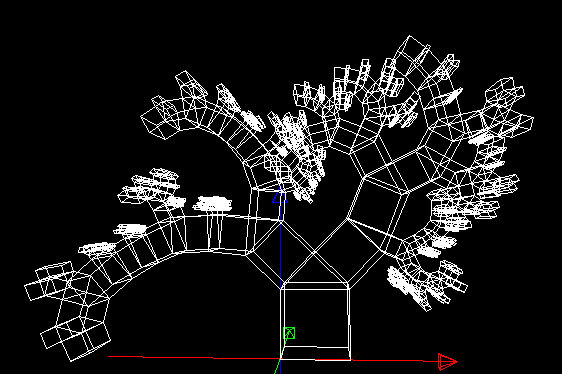
\includegraphics[width=\linewidth]{./pictures/seriell_randomWinkel_Depth8.PNG}
    \captionof{figure}{Pythagoras-Baum mit zufälligen Winkeln.\\Ebenen: 8}
    \label{fig:BaumRandomAngle}
\end{minipage}
\hfill
\begin{minipage}{0.45\linewidth}
    \centering
    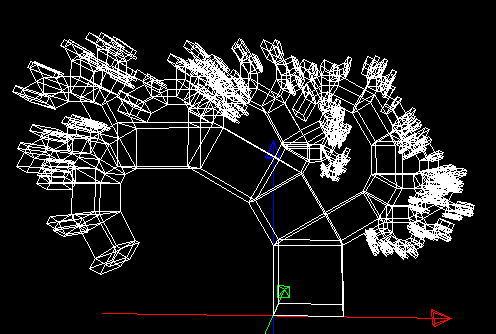
\includegraphics[width=\linewidth]{./pictures/seriell_randomHeight_Depth8.PNG}
    \captionof{figure}{Pythagoras-Baum mit zufälligen Quadern.\\Ebenen: 8}
    \label{fig:BaumRandomHeight}
\end{minipage}

\vspace{0.25cm}
\noindent
Besonders vielfältige Ergebnisse lassen sich erzielen, wenn man zufällige Winkel und zufällige Höhen kombiniert:
\vspace{0.1cm}\\
\noindent
\begin{minipage}{0.45\linewidth}
    \centering
    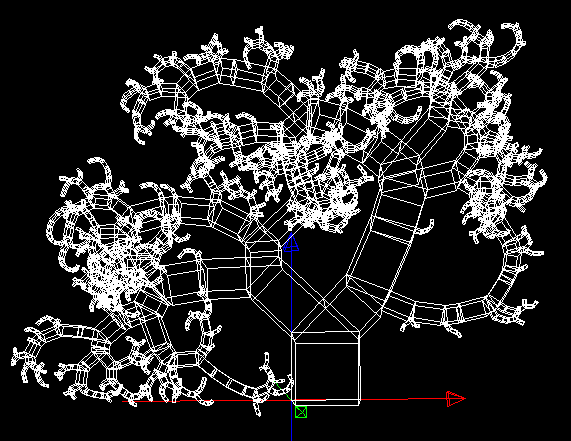
\includegraphics[width=\linewidth]{./pictures/Seriell-random_0.1.PNG}
    \captionof{figure}{Randomisierter Pythagoras-Baum. \\Minmale Seitenlänge: 0.1}
    \label{fig:BaumRandom1}
\end{minipage}
\hfill
\begin{minipage}{0.45\linewidth}
    \centering
    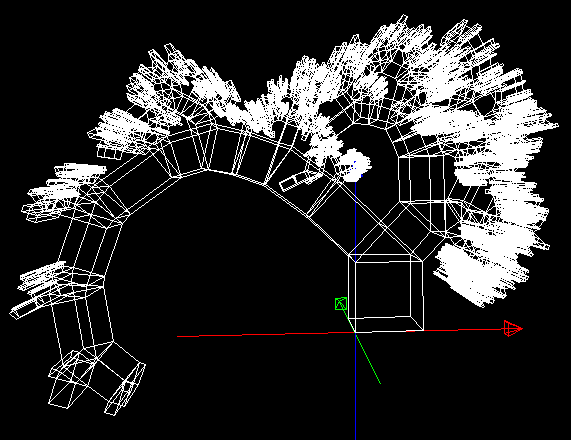
\includegraphics[width=\linewidth]{./pictures/seriell-random_Depth12.PNG}
    \captionof{figure}{Randomisierter Pythagoras-Baum.\\Ebenen: 12}
    \label{fig:BaumRandom2}
\end{minipage}

\newpage
\section{Parallele Realisierung}
Nachdem die serielle Implementierung zufriedenstellende Ergebnisse lieferte, konnten wir uns dem übergeordneten Ziel widmen unser 
Programm zu parallelisieren.\newline
Strukturell besteht ein Pythagoras-Baum aus einer Menge von Daten --- in unserem Fall Cuboid-Objekten ---
auf die immer wieder dieselbe Operation angewendet wird. Es handelt sich also um eine Datenparallelität. Aufgrund der linearen Speicherung
in einem Array beziehungsweise einem Vektor benötigen wir nur eine Dimension.\newline
Zwischen den Quadern einer Ebene bestehen keinerlei Abhängigkeiten. Dementsprechend ist eine Kommunikation oder Synchronisierung zwischen den einzelnen
Berechnungseinheiten generell nicht notwendig. 

\subsection{OpenCL}
\vspace{-0.25cm}
Unser erster Schritt war die Parallelisierung unter Verwendung der GPU. Da nur einer der verwendeten Laptops (Thinkpad P15) über eine 
Nvidia-Grafikkarte verfügte, fiel unsere Wahl auf OpenCL als Schnittstelle.\\
Grundsätzlich konnten wir eine zu unserer seriellen iterativen Funktion äquivalente Lösung implementieren --- es waren jedoch umfassende
Änderungen in unserem Programm notwendig. Da OpenCL reinen C-Code statt des bisher verwendeten C++ benötigte, mussten alle geschriebenen
C++-Klassen in C-Structs umgewandelt werden. In den für OpenCL relevanten Funktionen mussten wir außerdem auf den Einsatz von Funktionen
aus der C++ Standardbibliothek verzichten. \\
Eine zusätzliche Herausforderung war, dass alle im OpenCL-Kernel genutzten Funktionen direkt in der kernel.cl implementiert werden
mussten, wodurch eine große und unübersichtliche Datei entstand. 

\vspace{0.25cm}
Ähnlich wie bei der sequentiellen Version implementierten wir auch für die Umsetzung mit OpenCL eine Funktion 
\lstinline{generateWithOpenCL()}. Diese ruft die verfügbaren OpenCL Plattformen und Geräte ab und wählt die GPU als OpenCL device aus. 
Daraufhin wird ein Kontext und eine Command Queue erstellt, bevor der OpenCL-Kernel aus der kernel.cl eingelesen und kompiliert
wird. \\
Für die Berechnung der für den Baum benötigten Quader auf der GPU entschieden wir uns für einen feingranularen Ansatz, bei
welchem jeder Thread für genau einen Quader zuständig ist. Resultierend daraus war die Anzahl der benötigten GPU-Threads nicht vorab
festlegbar, weil sie sich mit jeder Ebene verdoppelte.
Grundsätzlich wäre eine feinere Granulierung möglich, indem beispielsweise
jeder Thread die Transformation eines einzelnen Punktes vornimmt --- hierbei wäre jedoch der Aufwand, die Daten sinnvoll zu verteilen
und anschließend korrekt wieder zusammenzufügen, exponentiell höher.\\
Zur Übermittlung des Vektors mit den bereits vorhandenen Quadern an die GPU und zum Zurückliefern des Arrays mit den erzeugten Quadern
nach Vollendung der Berechnungen an die CPU implementierten wir ein Double-Buffering-System\footnote{Double-Buffering = Verwendung 
zweier Buffer, die abwechselnd gefüllt werden, um Verzögerungen durch das Leeren und Löschen von Daten zu vermeiden}. 
Die Buffer werden vor dem Aufruf des Kernelcodes in unserer \lstinline{generateWithOpenCL()}-Funktion angelegt und auf die GPU übertragen. 

\subsubsection*{Näherungsfunktionen auf der GPU}
\vspace{-0.25cm}
Wie wir in der Vorlesung gelernt haben, haben Näherungsfunktionen wie Potenzen, Wurzeln oder auch trigonometrische Funktionen einen
negativen Einfluss auf die Performance von auf der GPU ausgeführten Programmen. Im Pythagoras-Baum kommen nicht nur Potenzen (welche
im benötigten Rahmen problemlos durch Multiplikationen ersetzbar waren) und Wurzeln, sondern vor allem auch Sinus- und Cosinusberechnungen 
zum Einsatz.\\
Initial planten wir, eine Sinus-Lookup-Table auf der CPU zu erstellen und diese als Buffer an die GPU zu übergeben. Unsere Recherche ergab
jedoch, dass dieser Ansatz auf der GPU bereits umgesetzt wird. Stattdessen wird die Verwendung von \texttt{native\_sin()} und
\texttt{native\_cos()} empfohlen. Die \glqq native\grqq-Funktionen liefern Näherungen mit für unsere Zwecke akzeptabler Genauigkeit und benötigen
maßgeblich weniger Laufzeit als die herkömmlichen \texttt{sin()}- und \texttt{cos()}-Funktionen.\footnote{Quellen (letzter Zugriff: 03.02.2026): 
\href{https://stackoverflow.com/questions/62546207/how-to-optimize-opencl-kernel-use-of-trigonometric-functions}{Stackoverflow - How to optimize OpenCL-Kernel use of trigonometric funktions} /
\href{https://registry.khronos.org/OpenCL/sdk/3.0/docs/man/html/erf.html}{khronos.org - OpenCL docs} /
\href{https://developer.download.nvidia.com/compute/DevZone/docs/html/OpenCL/doc/OpenCL_Best_Practices_Guide.pdf}{nvidia.com - OpenCL Best Practices Guide}}
Ein Nachteil dieses Ansatzes liegt in der limitierten Verfügbarkeit --- die \texttt{native}-Funktionen sind nicht auf allen
Rechnern respektive nicht bei allen OpenCL-Implementierungen verfügbar.\\
Darüber hinaus reduzierten wir die Menge der trigonometrischen Berechnungen, indem wir die Sinus- und Cosinus-Werte
für die Berechnung der Punkt-Transformation einmalig zu Beginn der Funktion berechneten, statt sie mehrfach neu zu kalkulieren. 
Auf einem Rechner mit Nvidia-GPU erreichten wir so eine Beschleunigung von bis zu 40\%. 
% https://stackoverflow.com/questions/62546207/how-to-optimize-opencl-kernel-use-of-trigonometric-functions

% https://registry.khronos.org/OpenCL/sdk/3.0/docs/man/html/erf.html
% A subset of functions from Built-in Scalar and Vector Argument Math Functions that are defined 
% with the native_ prefix. These functions may map to one or more native device instructions and 
% will typically have better performance compared to the corresponding functions without the native_ prefix). 
% The accuracy (and in some cases the input range(s)) of these functions is implementation-defined.

% https://developer.download.nvidia.com/compute/DevZone/docs/html/OpenCL/doc/OpenCL_Best_Practices_Guide.pdf
% Two types of runtime math operations are supported. They are
% native_functionName() and functionName(). Functions using
% native_functionName() map directly to the hardware level. They are faster but
% provide somewhat lower accuracy. (Examples: native_sin(x), native_exp(x),
% and so forth.) Functions using functionName() are slower but have higher
% accuracy. (Examples: sin(x), exp(x), and so forth.) The throughput of
% native_sin(x), native_cos(x), native_exp(x) is 1 operation per clock cycle,
% while sin(x), cos(x), tan(x) are much more expensive and become even more so
% (about an order of magnitude slower) if the absolute value of x needs to be reduced.
% Moreover, in such cases, the argument-reduction code uses local memory, which
% can affect performance even more because of the high latency of local memory.
% More details are available in the NVIDIA OpenCL Programming Guide.

% NOCH NICHT GELESEN ABER EVENTUELL LESENSWERT: 
% https://ijecce.org/administrator/components/com_jresearch/files/publications/IJECCE-3291_Final.pdf

\vspace{-0.25cm}
\subsubsection*{Zufallsbäume auf der GPU}
\vspace{-0.25cm}
Die Verwendung von Funktionen aus der C++ Standardbibliothek ist in OpenCL nicht möglich 
und das Erzeugen von Zufallszahlen auf der GPU generell problematisch. Daher mussten wir für das Generieren
zufälliger Bäume mit OpenCL die Zufallszahlen vorab auf der CPU erzeugen und an die GPU übergeben.\\
Glücklicherweise ließ sich die hierfür aufzubringende Zeit einfach minimieren, indem wir nur eine kleine Menge
Zahlen kalkulierten, die im Laufe der Berechnungen auf der GPU wiederverwendet werden konnten.
Theoretisch wäre eine Primzahl als Menge von Zufallszahlen vermutlich optimal. Wir erzielten jedoch auch mit 42 
Zufallszahlen schon Ergebnisse, die visuell einen guten Eindruck von Zufälligkeit erweckten. 
\vspace{0.5cm}\\
\begin{minipage}{0.49\linewidth}
   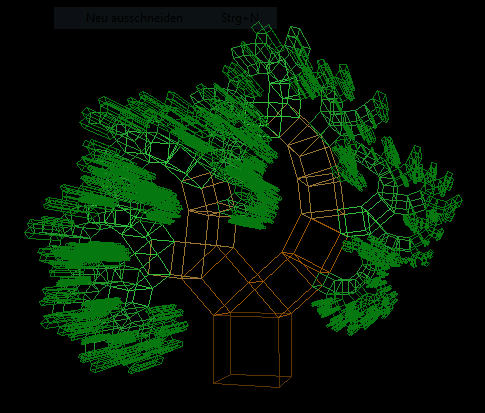
\includegraphics[width=\linewidth]{pictures/OCL_random_Depth10.PNG}
   \captionof{figure}{Zufallsbaum mit 10 Ebenen generiert auf der GPU}
   \label{fig:GPU-Rand-1}
\end{minipage}
\hfill
\begin{minipage}{0.49\linewidth}
   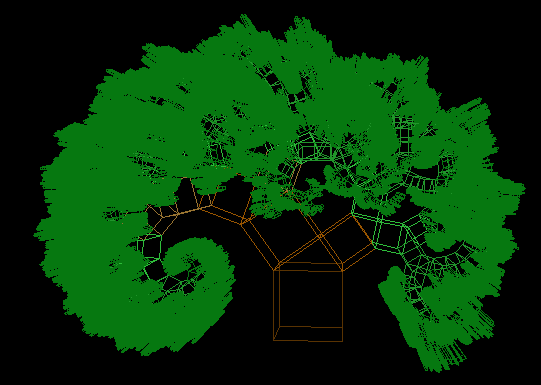
\includegraphics[width=\linewidth]{pictures/OCL_random_Depth18.PNG}
   \captionof{figure}{Zufallsbaum mit 18 Ebenen generiert auf der GPU}
   \label{fig:GPU-Rand-2}
\end{minipage}

% ----------------------------------- OpenMP ---------------------------------------
% ----------------------------------------------------------------------------------
\subsection{OpenMP}
\subsubsection*{Erzeugung einer Sinus-Lookup-Tabelle}
\vspace{-0.25cm}
Aufgrund der bekannten Problematik der Ineffizienz trigonometrischer Funktionen auf der GPU kam uns schon in der Planungsphase
unseres Projekts die Idee, mit OpenMP eine Sinus-Lookup-Tabelle zu berechnen. Diese sollte als Buffer auf die GPU übertragen
und dort bei den Berechnungen des \hyperref[Sinussatz]{Sinussatzes} und der Transformationsmatrizen verwendet werden.
Bevor wir feststellten, dass die GPU intern eine derartige Optimierung bereits verwendet, hatten wir eine erste Version dieses 
Ansatzes bereits implementiert. Dabei mussten wir jedoch feststellen, dass schon das sequentielle Befüllen des Arrays so schnell war,
dass eine Parallelisierung keinen Mehrwert geboten hätte.\\
Letztendlich entschieden wir uns dagegen, diese Idee weiter zu verfolgen.

\subsubsection*{Erzeugen von Pythagoras-Bäumen}
\vspace{-0.25cm}
Auch die mit OpenMP parallelisierte Implementierung in der Funktion \lstinline{generateWithOpenMP()} folgt demselben Konzept wie die sequentielle
iterative Funktion. Anders als für die Umsetzung von OpenCL mussten hierfür keine umfassenden Änderungen unseres Programms erfolgen. Da wir zur
iterativen Erstellung der Pythagoras-Bäume mit for-Schleifen arbeiten, konnten wir zur Parallelisierung das Pragma
\lstinline{#pragma omp parallel for} verwenden.\\
Um beim Sammeln der berechneten Quader im Result-Vektor keine Daten zu verlieren, arbeiteten wir anfangs mit einem kritischen Bereich. Diesen 
konnten wir durch Verwenden der durch die Laufvariable der for-Schleife vorgegebenen Indizes entfernen:
\vspace{0.25cm}\\
\begin{minipage}{0.58\linewidth}
\begin{lstlisting}[caption={Ausschnitt generateWithOpenMP(): Kritischer Bereich}]
...
 #pragma omp critical
 {
     resultCuboids.push_back(newCuboid_b);
     resultCuboids.push_back(newCuboid_a);
 }
...
\end{lstlisting}
\end{minipage}
\hfill
\begin{minipage}{0.35\linewidth}
\begin{lstlisting}[caption={Ersatz für kritischen Bereichs\\ i: Laufvariable for-Schleife}]
...
 resultCuboids[i*2+1] = newCuboid_b;
 resultCuboids[i*2] = newCuboid_a;
...
\end{lstlisting}
\end{minipage}
\vspace{0.25cm}\\
Das Generieren von Zufallsbäumen unter Nutzung von OpenMP stellte kein Problem dar. Ebenso wie in der sequentiellen Umsetzung konnte 
die \texttt{rand()}-Funktion aus der C++-Bibliothek eingesetzt werden.
\vspace{0.25cm}\\
Da auf der CPU in der Regel maximal acht oder 16 Kerne zur Verfügung stehen, ist die Parallelität hier deutlich grobgranularer als bei 
der GPU-Parallelisierung. Zwar verarbeiten wir nach wie vor jeden Quader einzeln, jedoch muss jeder CPU-Kern dabei eine große Menge Quader 
nacheinander berechnen. 

\begin{minipage}{0.49\linewidth}
   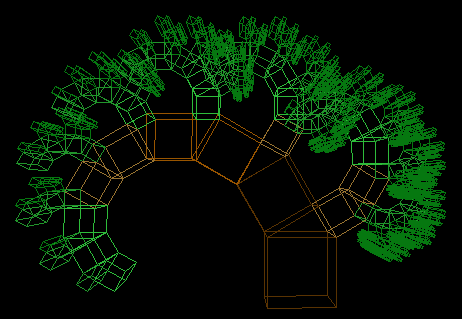
\includegraphics[width=\linewidth]{pictures/OMP_fixed_Depth8.PNG}
   \captionof{figure}{Pythagoras-Baum mit 8 Ebenen generiert mit OpenMP}
   \label{fig:OMP-fixed}
\end{minipage}
\hfill
\begin{minipage}{0.49\linewidth}
   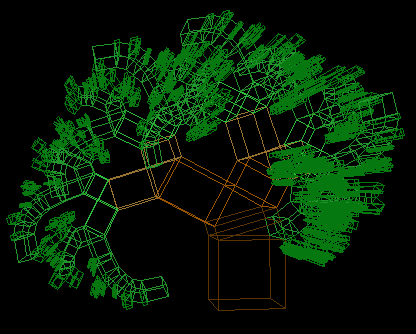
\includegraphics[width=\linewidth]{pictures/OMP_random_Depth10.PNG}
   \captionof{figure}{Zufallsbaum mit 10 Ebenen generiert mit OpenMP}
   \label{fig:OMP-random}
\end{minipage}

\subsubsection*{Hinzufügen von Objekten zum Renderer}\label{3-2-rendering}
\vspace{-0.25cm}
Die Quader des Pythagoras-Baums liegen nach ihrer Berechnung mit einer beliebigen Methode als Vektor vor und müssen einzeln
für den Renderer aufbereitet werden. Zwischen den verschiedenen Körpern bestehen keine Abhängigkeiten, sodass die umschließende for-Schleife
gut auf der CPU zu parallelisieren ist. Der Aufruf der Funktion \lstinline{addCuboidToRenderer()} zum Hinzufügen von Objekten zum Renderer erfolgt 
also parallelisiert. Daraus resultiert, dass auch bei der mit OpenCL parallelisierten und am Ende der sequentiellen Ausführung OpenMP zum Einsatz 
kommt, um die Gesamtlaufzeit des Programms zu verbessern.\\
Damit beim tatsächlichen Zugriff auf die Sammlung an Render-Objekten im Renderer Kollisionen verhindert werden, ist dieser separate Schritt als
kritischer Bereich markiert: 
\vspace{0.25cm}
\begin{lstlisting}[caption={Ausschnitt aus addCuboidToRenderer() mit kritischem Bereich}]
// Aufruf in main(): 
 #pragma omp parallel for
 for (Cuboid& c : cuboids) {
    addCuboidToRenderer(c, myRenderer);
 }

// Funktion: 
 void addCuboidToRenderer(const Cuboid &cube, Renderer& renderer) {
 ...
 #pragma omp critical
    renderer.addRenderObject(std::move(cubeObject));
 ...
 }
\end{lstlisting} 

% ----------------------------------- MPI ---------------------------------------
% -------------------------------------------------------------------------------
\newpage
\subsection{MPI}
\subsubsection{Konzeption}
\vspace{-0.25cm}
Analog zu den Implementierungen der bereits umgesetzen Funktionen sollte eine Funktion \lstinline{generateWithMPI()}
angelegt werden. Diese nimmt ein Inputarray mit mindestens einem Startquader sowie eine gewünschte Tiefe entgegen.\\
Zur parallelen Verarbeitung muss das Inputarray gleichmäßig auf die verfügbaren Rechner aufgeteilt werden. Prinzipiell kann
die Aufteilung da es keine Abhängigkeiten zwischen den Quadern gibt in n Sub-Arrays der Größe 
\[\frac{\text{Anzahl Inputquader}}{\text{Anzahl Prozesse}}
\quad \text{mit Anzahl Inputquader} = \text{inputarray.length()}
\]
erfolgen --- hierbei muss jedoch darauf geachtet werden, dass keine Quader übrig bleiben, wenn die Rechnung keine ganze Zahl ergibt. 
Anschließend kann jeder MPI-Prozess für seinen Teil der Inputquader die Folgequader berechnen.\\
Um nach Vollendung der Berechnungen wieder ein vollständiges Array mit allen Quadern zu erhalten, welches man an eine zentrale Instanz
zurückliefern kann, kann die MPI-Gather Methode zum Einsatz kommen.

\subsubsection{Umsetzung}
\vspace{-0.25cm}
Es ist zu erwarten, dass bei MPI dieselbe Problematik wie bei OpenCL durch das Umkopieren der Daten entstünde. Besonders dadurch, dass
der Transfer nicht länger innerhalb eines Rechners, sondern über das Netzwerk erfolgen müsste, gäbe es einen großen Overhead, der einen
Zeitgewinn unwahrscheinlich macht.\\
Darüber hinaus bliebe unser in \hyperref[Speicher]{Kapitel 5.4} detailliert aufgeführtes Speicherplatzproblem bestehen, weshalb 
eine Implementierung der MPI-Parallelisierung zum jetzigen Zeitpunkt keinen Mehrwert für die Laufzeit unseres Programms bieten kann.

% Chat-GPT:
% Overhead-Kosten:
%     MPI benötigt eine erhebliche Menge an overhead, um Prozesse zu starten und zu verwalten, was bei kleinen Datenmengen ineffizient sein kann.
% 
% Datenkommunikation:
%     Bei der Parallelisierung mit MPI wird die Kommunikation zwischen verteilten Prozessen über ein Netzwerk realisiert, was zusätzliche Latenzzeiten und Kommunikationsprobleme verursachen kann.
% 
% Anwendungsstruktur:
%     Der 3D Pythagorasbaum könnte in einer Einzel- oder Mehrkernumgebung effizienter umgesetzt werden, da die Datenlokalität und der Zugriff auf den gemeinsamen Speicher in einem Shared-Memory-System (wie bei OpenMP) besser unterstützt werden.
% 
% Einrichtungs- und Fehleraufwand:
%     MPI erfordert eine komplexere Setup- und Fehlerbehandlungslogik im Vergleich zu OpenCL und OpenMP, die in vielen Fällen nicht gerechtfertigt ist.
% 
% Keine signifikante Leistungsteigerung:
%     Wenn die zu verarbeitenden Daten oder die Berechnungen nicht ausreichend groß sind, kann MPI im Vergleich zu OpenCL oder OpenMP keine signifikante Leistungssteigerung bieten.
% 
% Portabilität und Zugänglichkeit:
%     Die Einführung von MPI könnte zusätzliche Anforderungen an die Hardware (z. B. mehrere Knoten oder Cluster) stellen, was die Portabilität und Zugänglichkeit für weniger erfahrene Benutzer einschränkt.
% 
% Eingeschränkte Parallelisierungsstrategien:
%     Da der Pythagorasbaum in einem rekursiven und hierarchischen Format data-parallelisiert wird, könnte die Verwendung von MPI zu einem Mangel an Flexibilität führen, da es primär für task-parallelistische Anwendungen konzipiert ist.

\subsection{Pattern und Operationen}
\vspace{-0.25cm}
Design-Pattern und vordefinierte Operationen helfen dabei, wiederkehrende programmatische Probleme bei der Parallelisierung eines Programms zu lösen.
Ein typisches Problem, auf welches wir während unserer Projektumsetzung stießen, war die ursprünglich rekursive sequentielle Funktion. Diese konnten
wir wie in \hyperref[iterativ]{Abschnitt 2.2} beschrieben unter Anwendung des Divide and Conquer Patterns\footnote{Divide and Conquer = Zerlegen eines Problems in Teilprobleme zur besseren Lösung} in eine 
iterative Version mit einer for-Schleife umwandeln. \\
Außerdem basiert die Generierung von Folgequadern aus den Inputquadern in unseren iterativen Umsetzungen auf einer Scatter-Operation. In jedem Schritt werden
aus einem eingelesenen Quader zwei Folgequader erzeugt.\\
Insgesamt tragen diese Strukturen dazu bei, die Komplexität des Codes zu reduzieren, die Last besser zu verteilen, die Skalierbarkeit zu erhöhen und so 
letztendlich die Laufzeit zu verbessern. 


\newpage
\section{Laufzeitvergleiche}
Zur Feststellung der Effizienz unserer Parallelisierungen haben wir die Laufzeit des Programms mit verschiedenen Parametern
aufgezeichnet. Um vergleichbare Ergebnisse zu erhalten, wurden alle Messungen mit einem festen Winkel von 30° und gleichen Höhen
(Höhe = Länge = Breite des Würfels mit einem Startwürfel der Seitenlänge 2) durchgeführt. 
Die Baumtiefe --- und damit die Anzahl zu berechnender Würfel --- wurde durch die Anzahl an Ebenen variiert.\\
Jeder Messwert in den folgenden Diagrammen wurde auf allen Geräten durch siebenfache Programmausführung und anschließendes
Bilden des Mittelwerts bestimmt (siehe \hyperref[Anhang]{Anhang}). Zur besseren Veranschaulichung wurden die Graphen in zwei Abschnitte unterteilt --- der 
erste Teil zeigt das Verhalten bei geringen Baumtiefen von fünf bis 13 Ebenen, der zweite Abschnitt für größere
Baumtiefen von 15 bis 21 Ebenen.

\vspace{-0.25cm}
\subsection{Sequentiell vs. OpenCL}
\vspace{-0.25cm}
Die folgenden Diagramme vergleichen die Laufzeit einer sequentiellen Ausführung mit einer durch OpenCL 
parallelisierten Ausführung.\\
Auf dem Thinkpad P15 wurde mit OpenCL je nach Baumtiefe eine Beschleunigung von etwa 40\% bis 87\% erreicht.
Allerdings trat diese erst bei Bäumen mit mehr als 16 Ebenen ein. Für Bäume mit nur fünf bis sieben Ebenen war OpenCL um 
den Faktor 120 - 360 langsamer als das sequentielle Pendant. 
\begin{figure}[H]
    \centering
    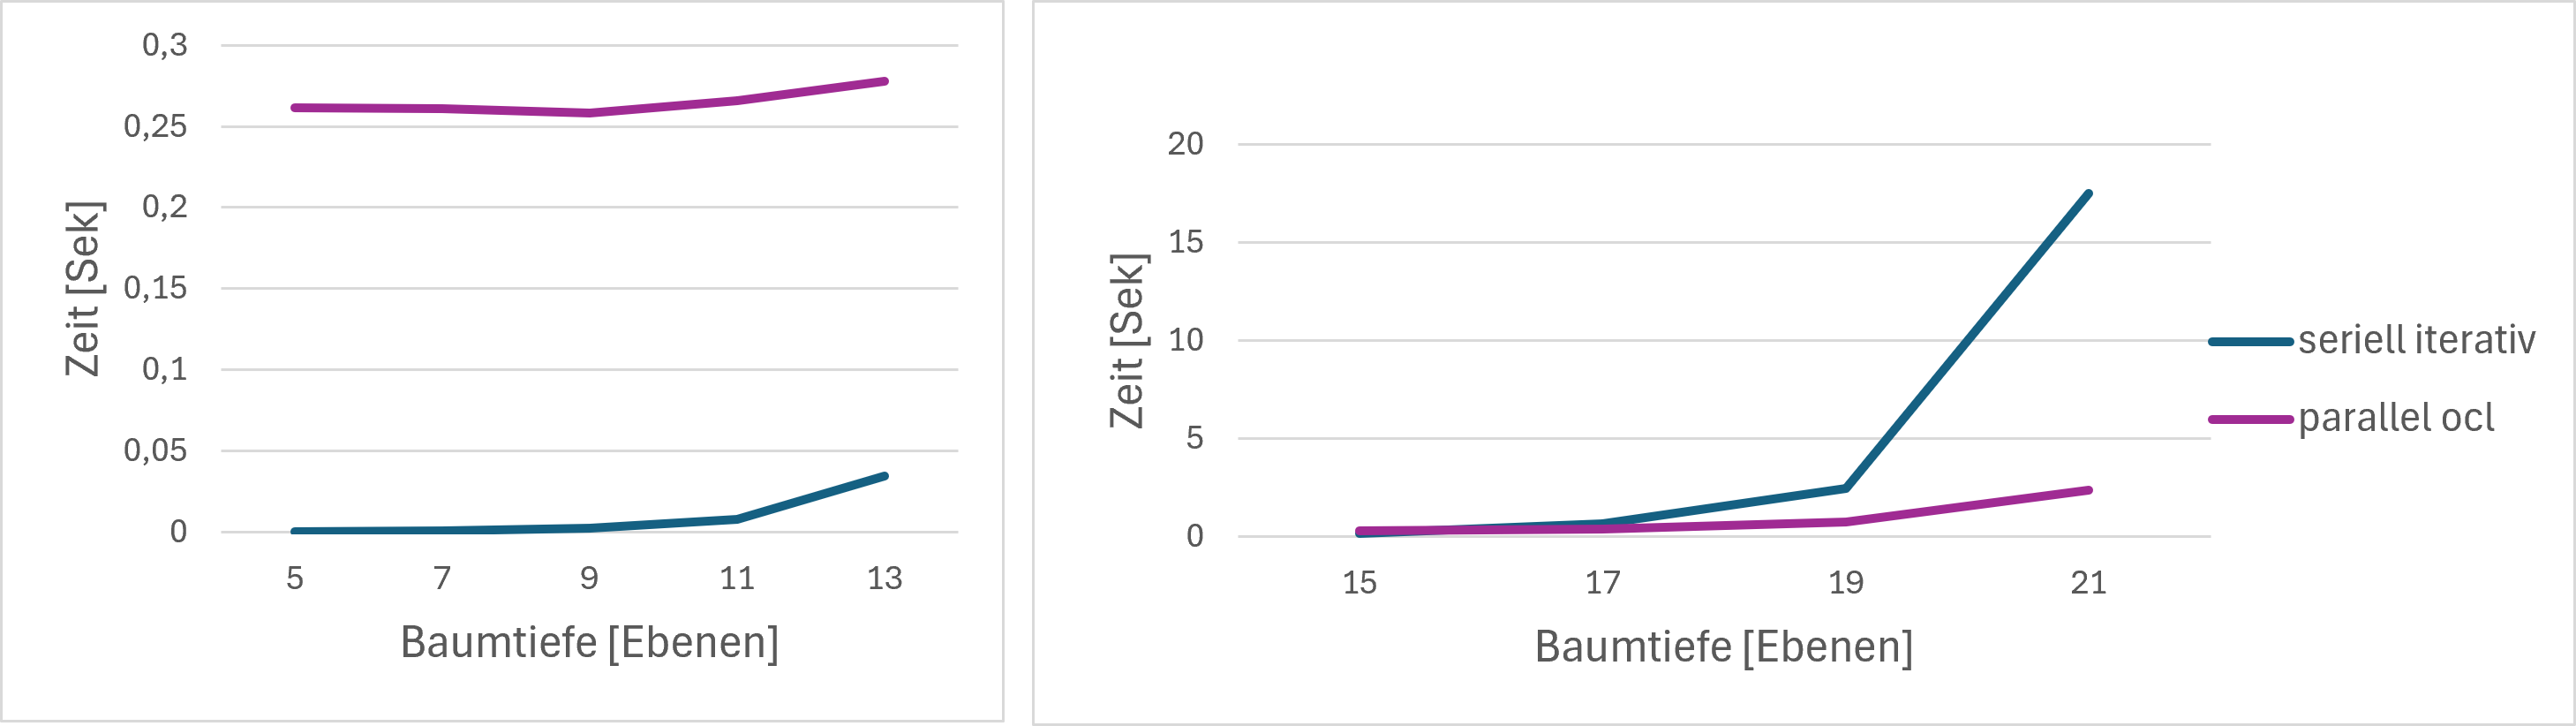
\includegraphics[width=0.9\linewidth]{./diagrams/seriellVsOCL_Tomke.png}
    \caption{Vergleich sequentielle vs. OpenCL Ausführung auf Thinkpad P15 Gen 2}
    \label{fig:seriellOCL1}
\end{figure}

\noindent Auf dem ASUS ZenBook war die OpenCL-Implementierung besonders für geringe Baumtiefen
ebenfalls deutlich im Nachteil. Für mittelgroße Bäume mit elf bis 17 Ebenen brauchte OpenCL etwa 2,5 bis 85x so 
lange wie die sequentielle Ausführung, bei sehr kleinen Bäume sogar zwischen etwa 300 und 
4000 Mal länger.
Erst ab einer Größe von 21 Ebenen zeigte sich ein Vorteil durch die Parallelisierung auf der GPU.
\begin{figure}[H]
    \centering
    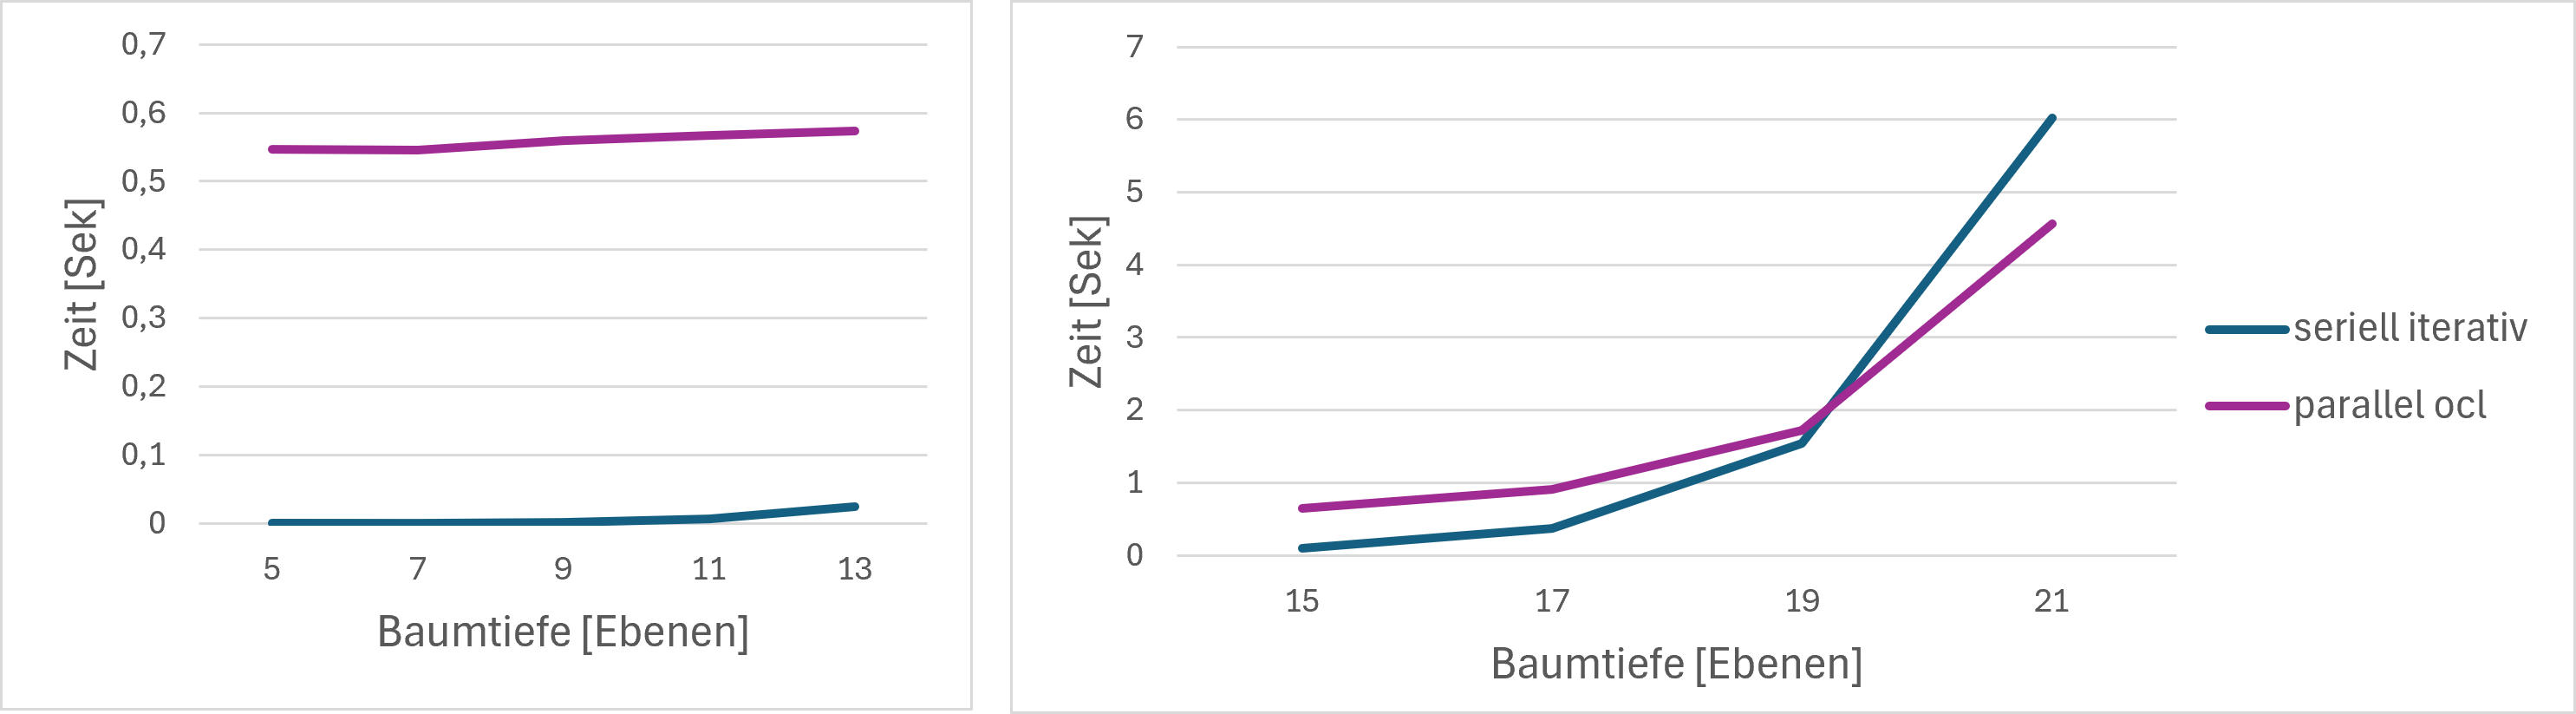
\includegraphics[width=0.9\linewidth]{./diagrams/seriellVsOCL_Sofie.png}
    \caption{Vergleich sequentielle vs. OpenCL Ausführung auf ASUS ZenBook 13}
    \label{fig:seriellOCL2}
\end{figure}

\noindent Anders als auf den anderen beiden Geräten war die Ausführung mit OpenCL auf dem Thinkpad P14s schon 
ab 15 Ebenen Baumtiefe deutlich schneller als die sequentielle Implementierung. Insgesamt konnte eine
Beschleunigung von 35\% - 88\% erreicht werden. Selbst für geringere Baumtiefen war die OpenCL-Ausführung im 
Vergleich zu der Ausführung auf den zuvor betrachteten Geräten schneller. Dennoch war OpenCL etwa 2x bis 375x 
langsamer als die sequentielle Implementierung.
\begin{figure}[H]
    \centering
    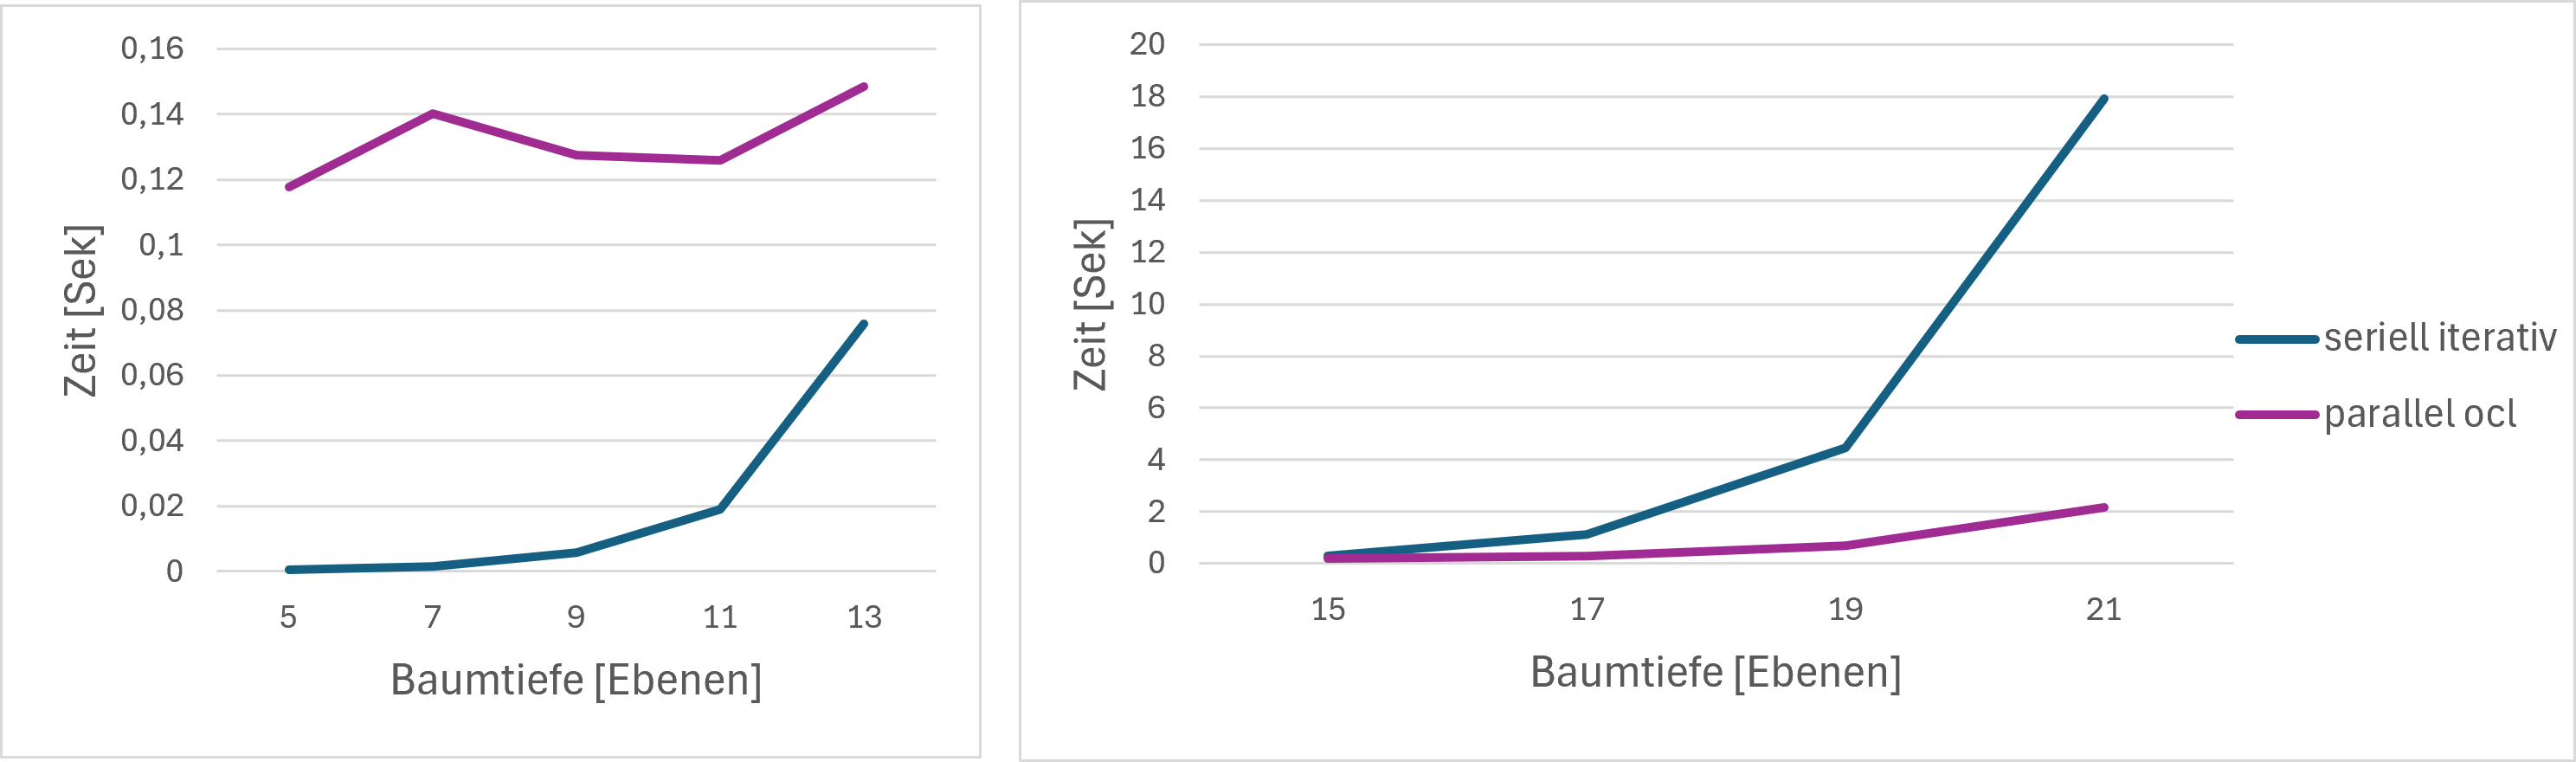
\includegraphics[width=0.9\linewidth]{./diagrams/seriellVsOCL_Patrick.png}
    \caption{Vergleich sequentielle vs. OpenCL Ausführung auf Thinkpad P14s Gen 1}
    \label{fig:seriellOCL3}
\end{figure}

\subsection{Sequentiell vs. OpenMP}
\vspace{-0.25cm}
Im nächsten Schritt haben wir die Ausführungszeiten unserer sequentiellen Implementierung denen der Parallelisierung
mit OpenMP gegenübergestellt.\\
Hierbei war OpenMP auf dem Thinkpad P15 für Bäume mit fünf bis sieben Ebenen zwar etwa doppelt so langsam wie die sequentielle 
Implementierung, konnte die Ausführung bei Bäumen mit elf oder mehr Ebenen aber zwischen 50\% und 93\% Zeitersparnis erwirken.
\begin{figure}[H]
    \centering
    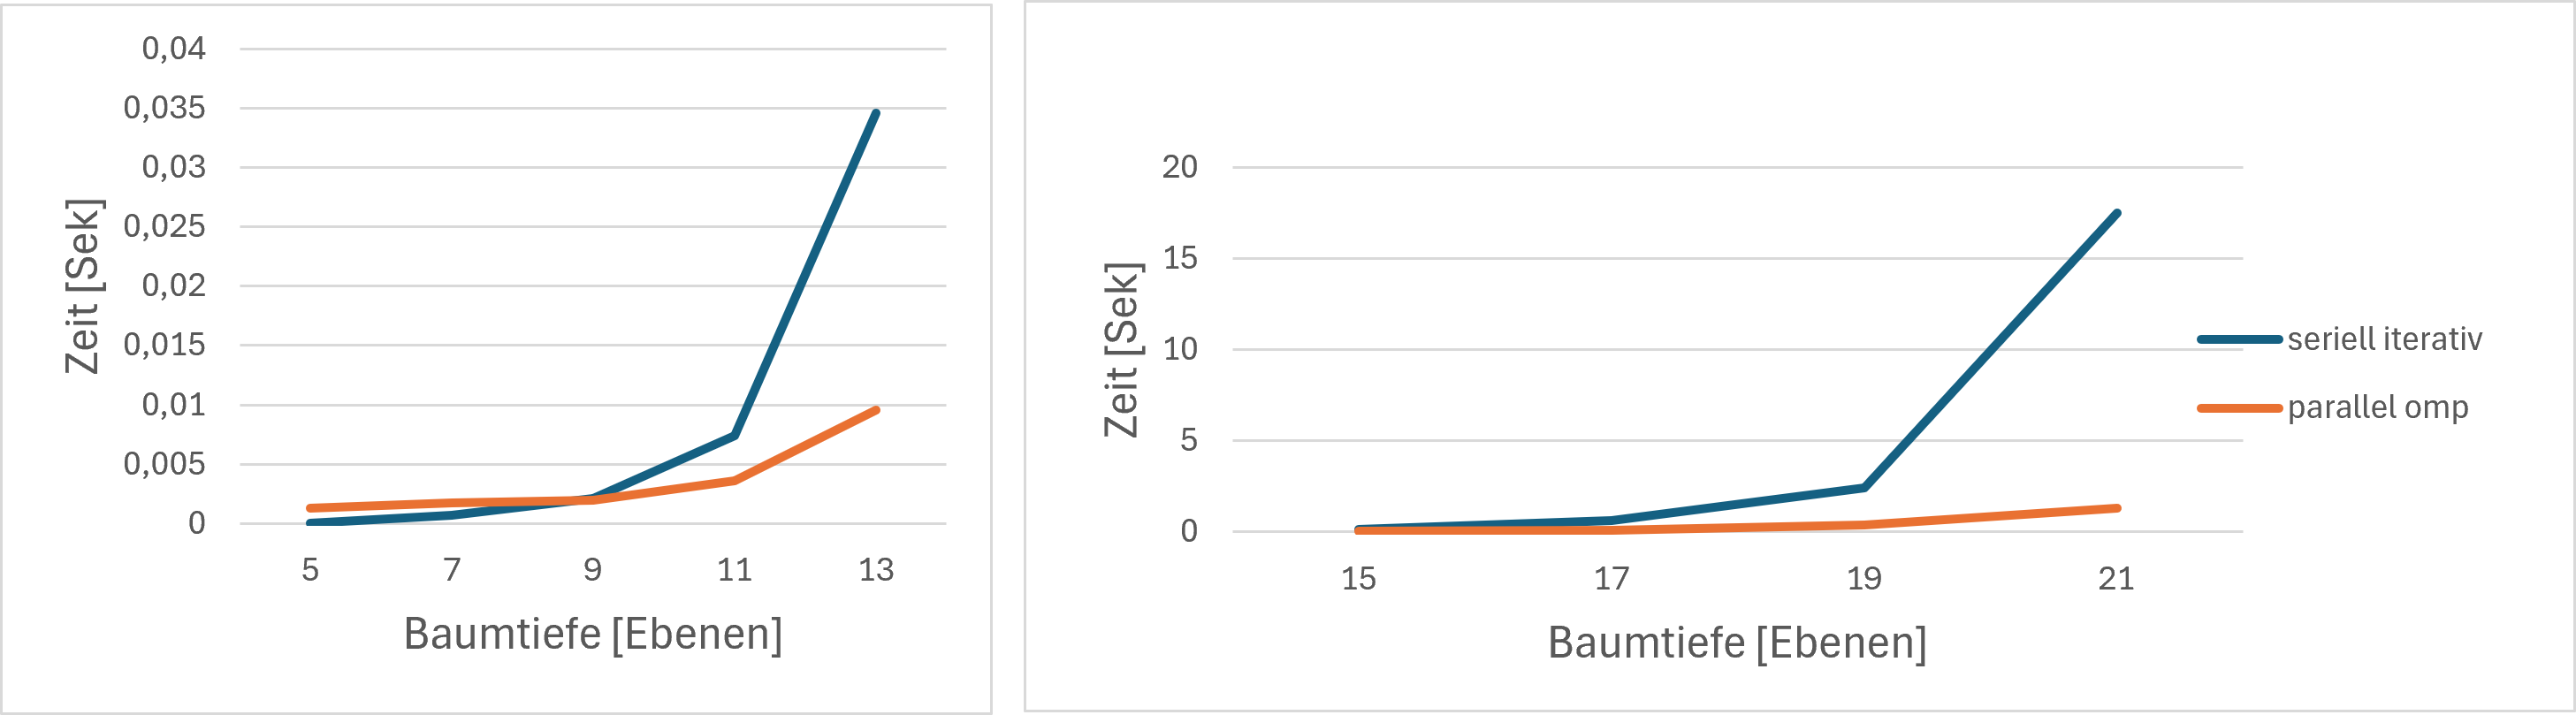
\includegraphics[width=\linewidth]{./diagrams/seriellVsOMP_Tomke.png}
    \caption{Vergleich sequentielle vs. OpenMP Ausführung auf Thinkpad P15 Gen 2}
    \label{fig:seriellOMP1}
\end{figure}

\noindent Auch auf dem ASUS ZenBook konnte ab elf Ebenen Baumtiefe eine Beschleunigung von 50\% festgestellt werden. Die höchste 
Zeitersparnis lag bei 80\%. Für kleine Bäume war die sequentielle Implementierung um einen Faktor von 1,5 bis 6 zeiteffizienter.
\begin{figure}[H]
    \centering
    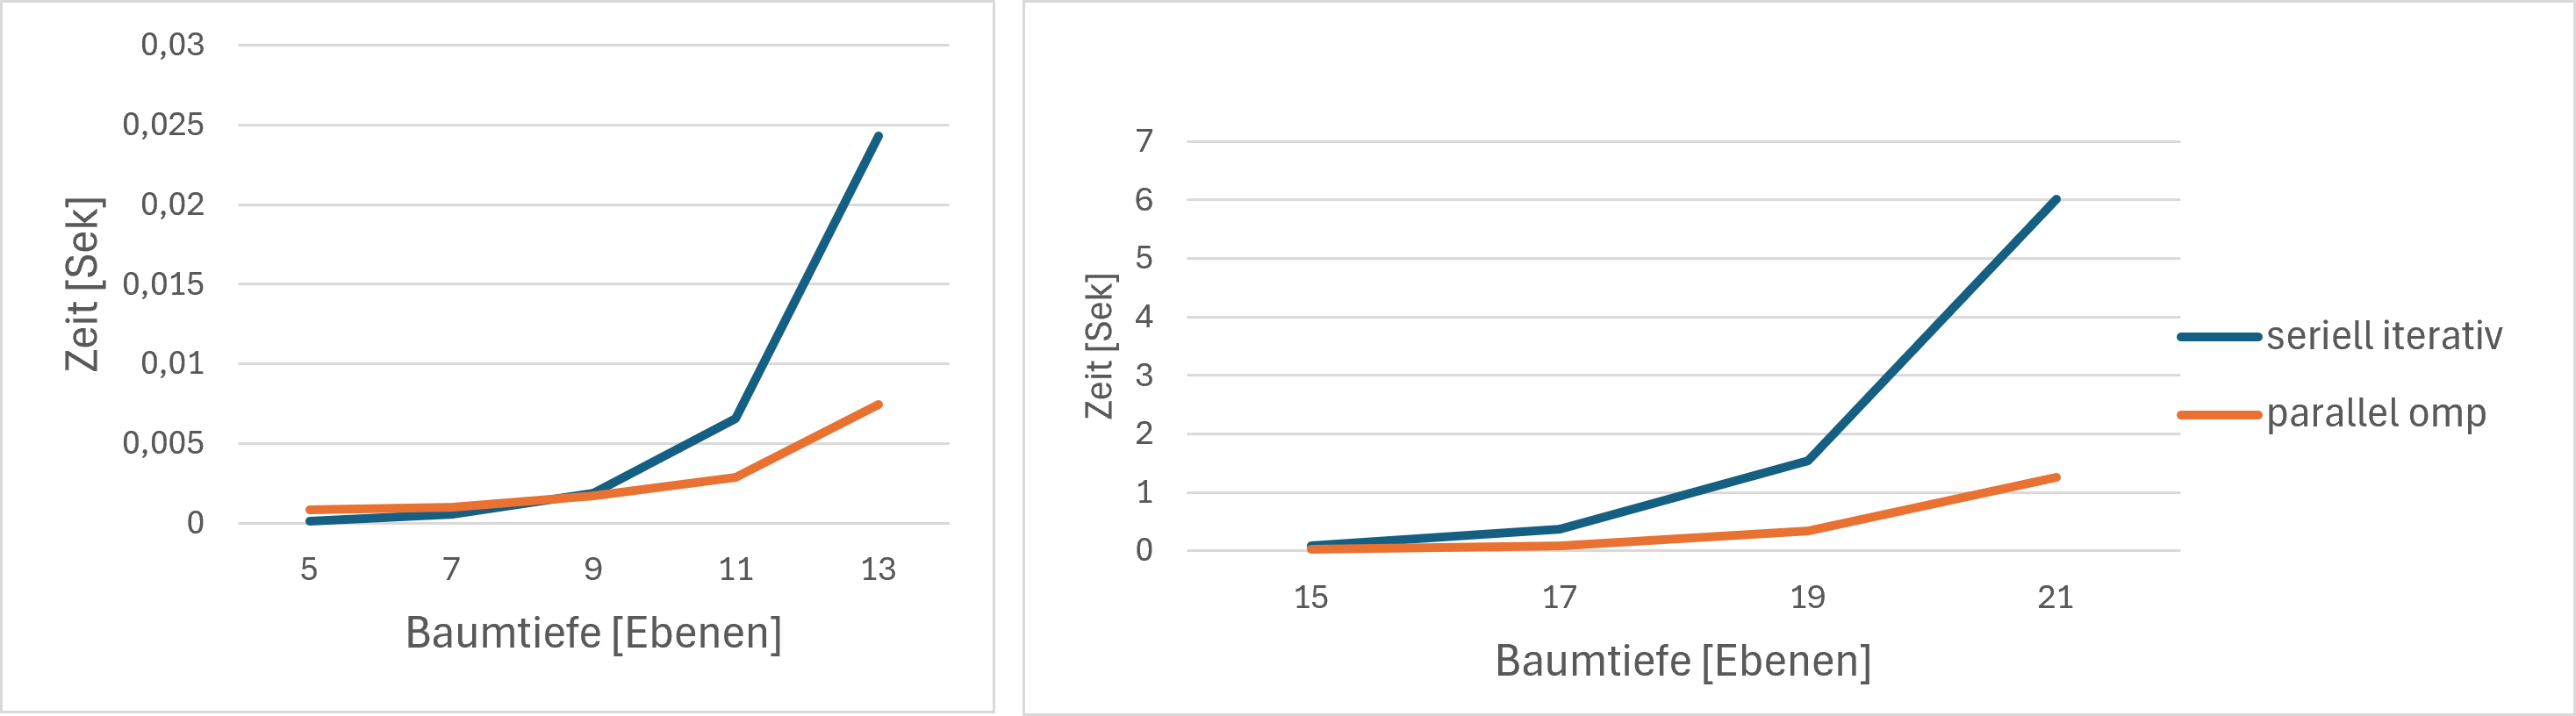
\includegraphics[width=\linewidth]{./diagrams/seriellVsOMP_Sofie.png}
    \caption{Vergleich sequentielle vs. OpenMP Ausführung auf ASUS ZenBook 13}
    \label{fig:seriellOMP2}
\end{figure}

\noindent Deutlich schlechter waren die für OpenMP gemessenen Zeiten für kleine Bäume auf dem Thinkpad P14s. Hier war die sequentielle Ausführung 
zwischen drei und 30x schneller. Dafür konnte eine Beschleunigung mit Faktor zwei durch die Parallelisierung schon bei neun Ebenen 
erwirkt werden. Insgesamt war eine Beschleunigung von bis zu 80\% möglich.
\begin{figure}[H]
    \centering
    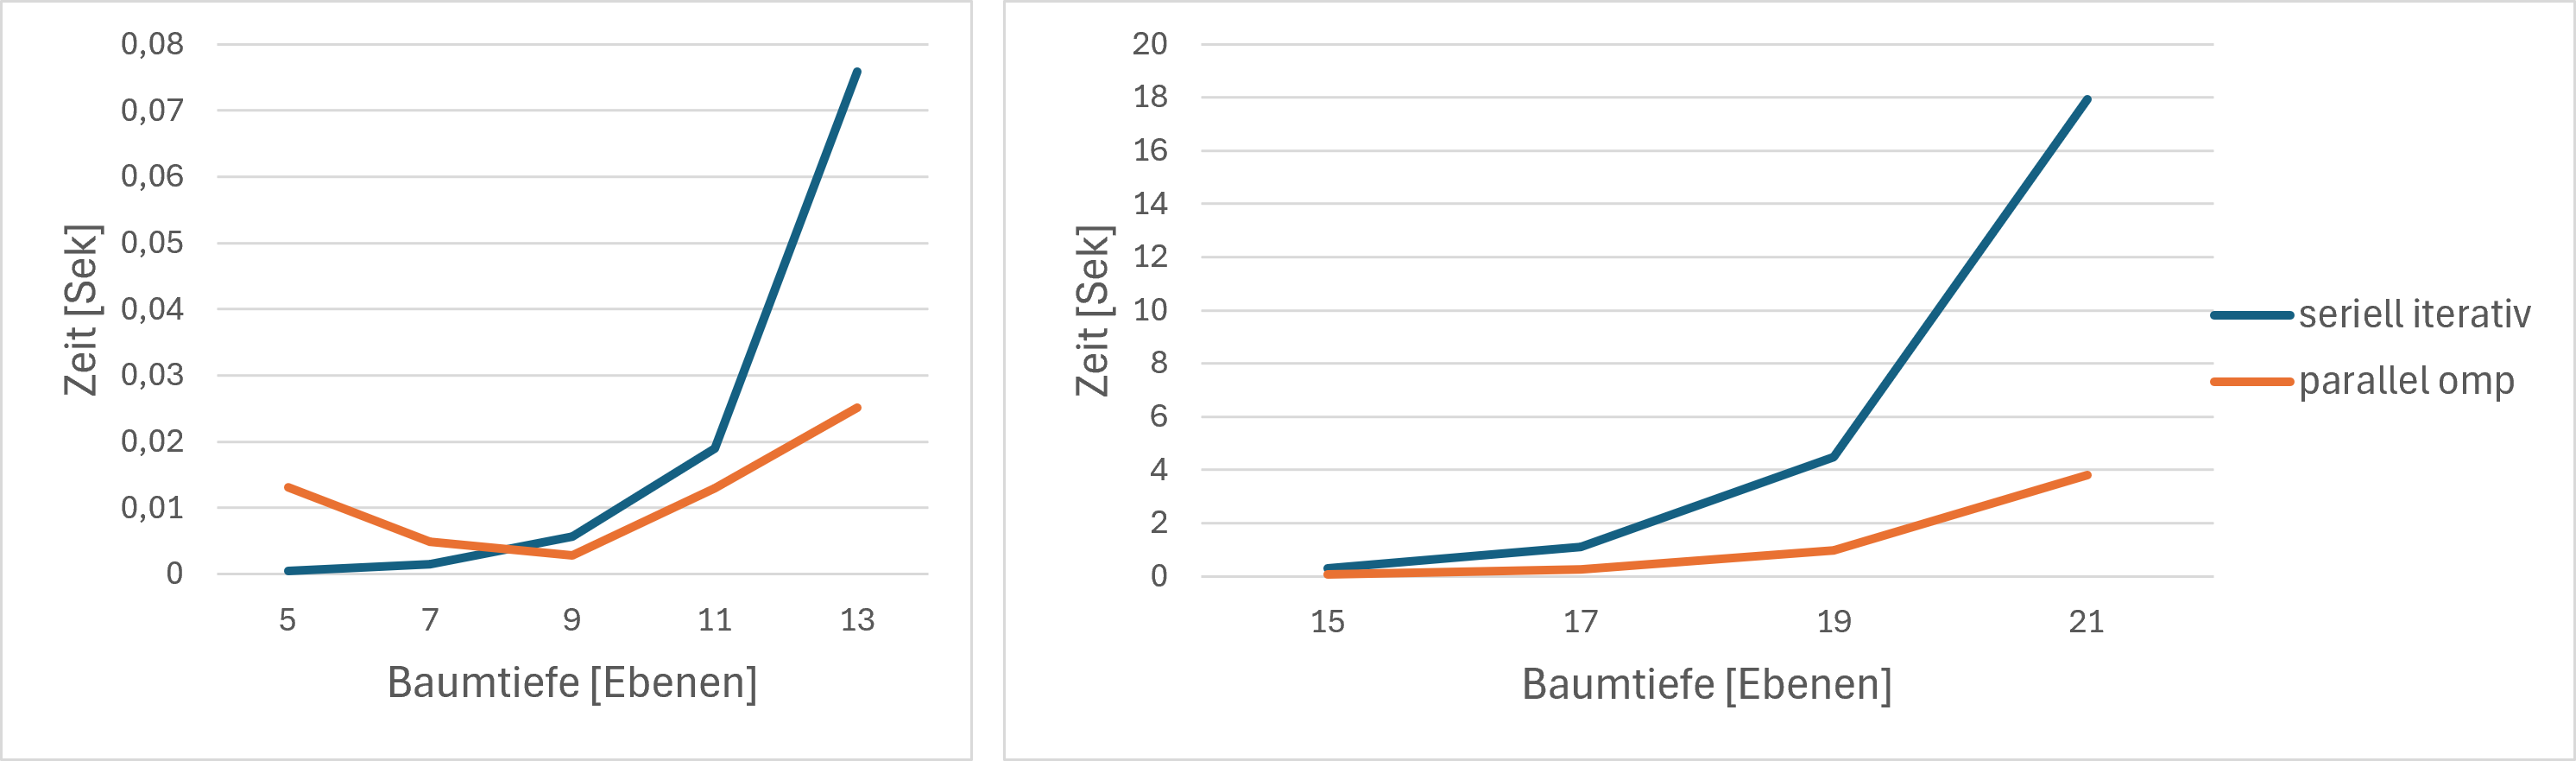
\includegraphics[width=\linewidth]{./diagrams/seriellVsOMP_Patrick.png}
    \caption{Vergleich sequentielle vs. OpenMP Ausführung auf Thinkpad P14s Gen 1}
    \label{fig:seriellOMP3}
\end{figure}

\subsection{OpenCL vs. OpenMP}
\vspace{-0.25cm}
Um einen Eindruck über die bestmögliche Beschleunigung unseres Programms zu gewinnen, haben wir zuletzt auch die beiden parallelen 
Technologien, OpenCL und OpenMP, gegenübergestellt.\\
Während auf dem Thinkpad P15 und dem ASUS ZenBook OpenCL deutlich langsamer war als OpenMP --- Faktoren zwischen 2 und 630 --- war
auf dem Thinkpad P14s ab 19 Ebenen OpenCL um 30 - 45\% schneller.
\vspace{0.5cm}\\
\begin{minipage}{0.49\linewidth}
    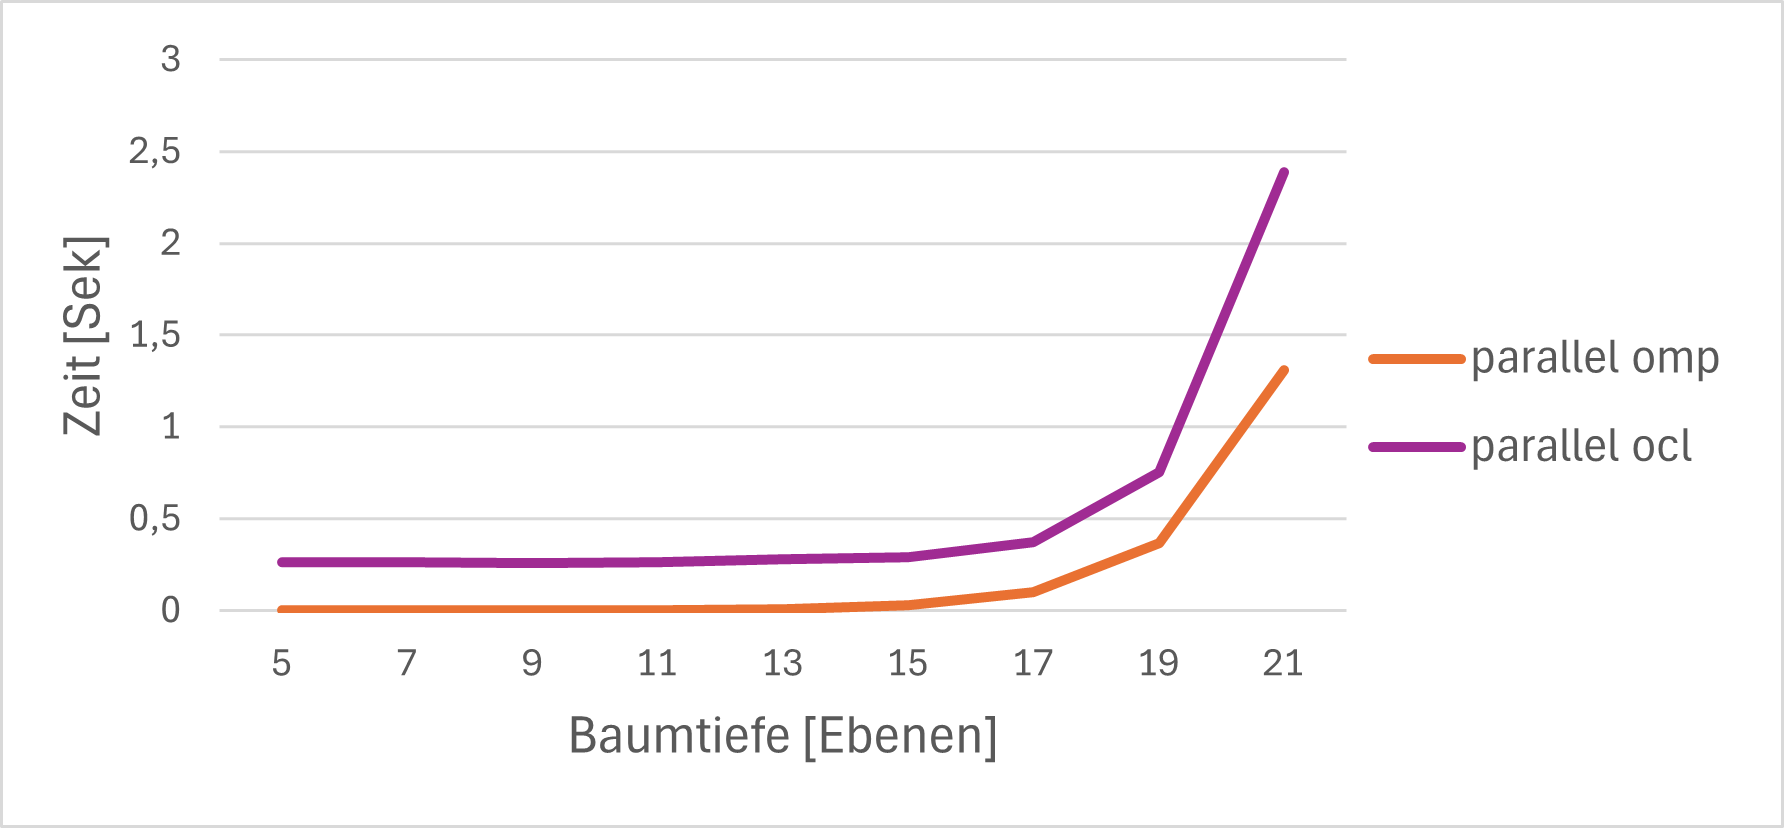
\includegraphics[width=\linewidth]{./diagrams/ompVsOCL_Tomke.png}
    \captionof{figure}{Vergleich OpenMP vs. OpenCL Ausführung auf Thinkpad P15 Gen 2}
    \label{fig:ocl-opm-1}
\end{minipage}
\hfill
\begin{minipage}{0.49\linewidth}
    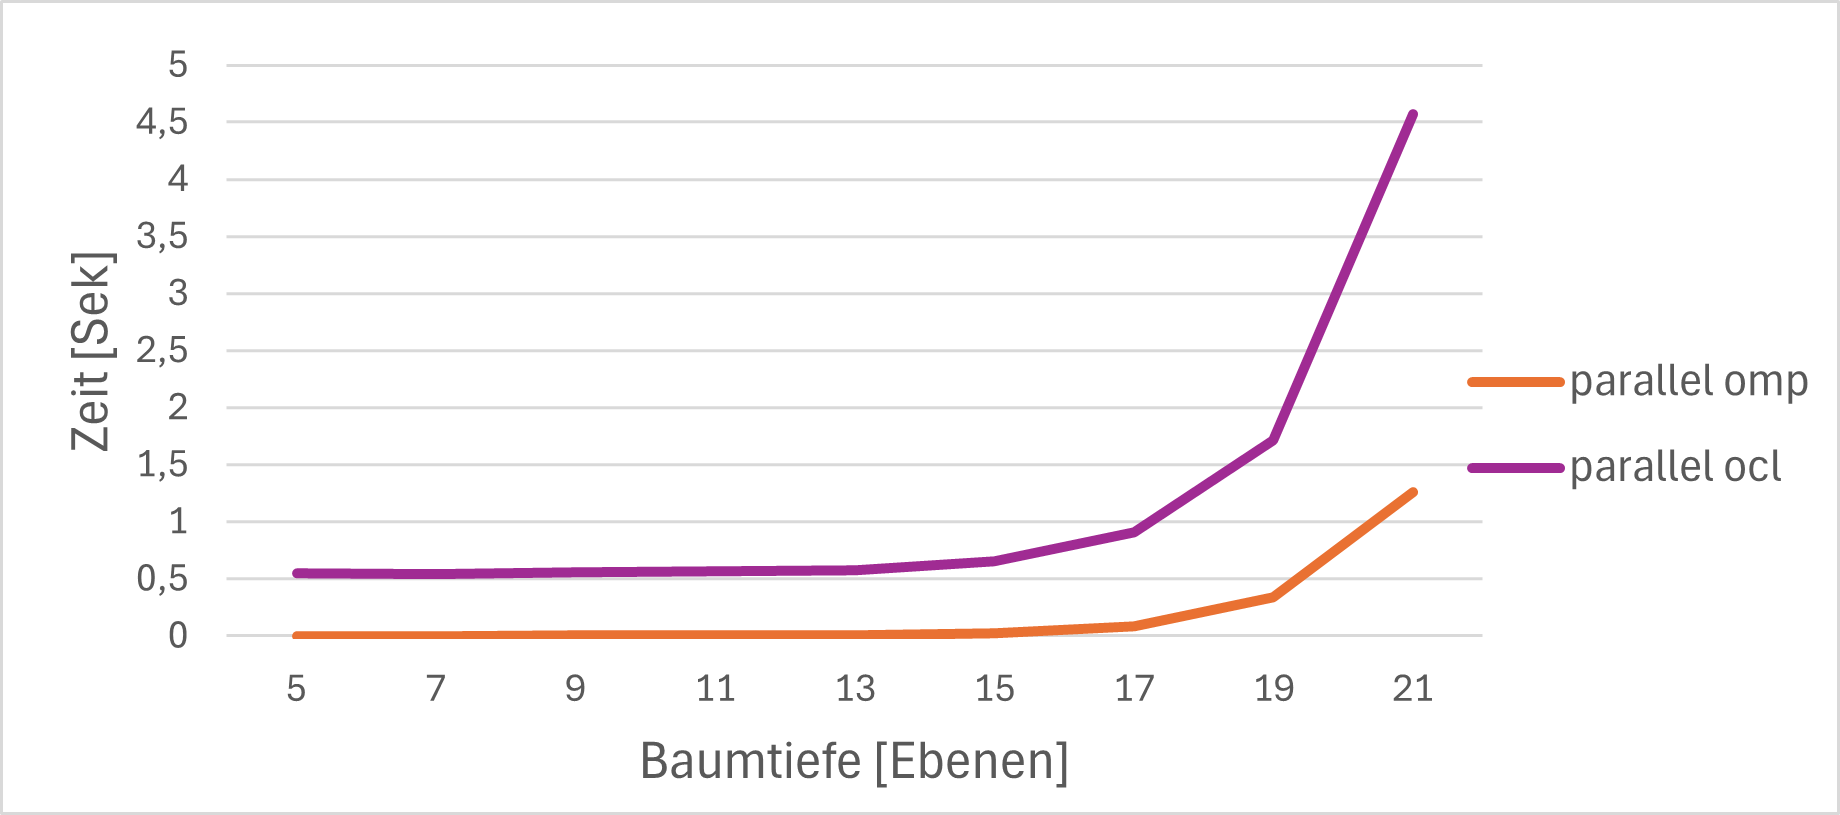
\includegraphics[width=\linewidth]{./diagrams/ompVsOCL_Sofie.png}
    \captionof{figure}{Vergleich OpenMP vs. OpenCL Ausführung auf ASUS ZenBook 13}
    \label{fig:ocl-opm-2}
\end{minipage}
\begin{figure}[H]
    \centering
    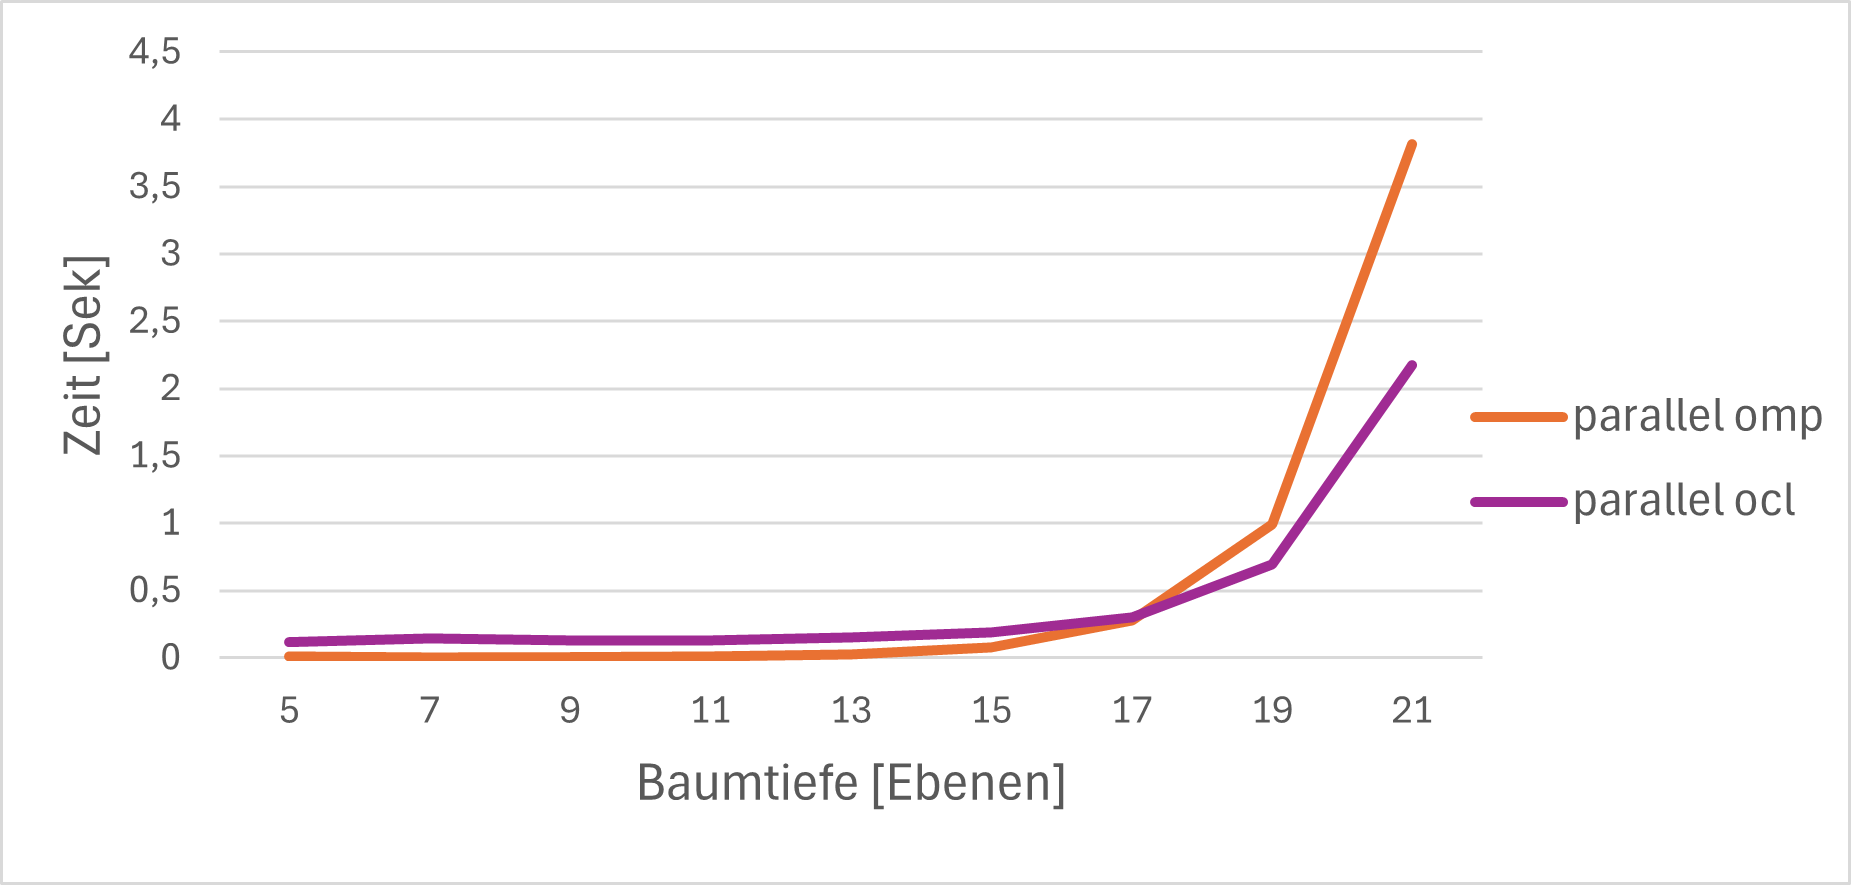
\includegraphics[width=0.5\linewidth]{./diagrams/ompVsOCL_Patrick.png}
    \caption{Vergleich OpenMP vs. OpenCL Ausführung auf Thinkpad P14s Gen 1}
    \label{fig:ocl-opm-1}
\end{figure}

\vspace{0.25cm}
\noindent Der erhebliche zeitliche Nachteil, welchen OpenCL vor allem bei geringen Baumtiefen aufweist, lässt
sich durch den Overhead erklären der entsteht, weil die zu verarbeitenden Daten --- das Array mit den Quadern --- über
den Systembus aus dem Arbeitsspeicher der CPU in den Grafikkarteneigenen RAM kopiert werden müssen.\\
Hiermit ist auch zu begründen, dass die für die OpenCL-Ausführung gemessenen Zeiten auf dem Thinkpad P14s deutlich schneller
sind. Durch die Verwendung von PoCL müssen die Daten nur innerhalb der CPU kopiert werden, was eine erhebliche Zeitersparnis 
mit sich bringt.

\vspace{0.5cm}
\begin{minipage}{0.49\linewidth}
    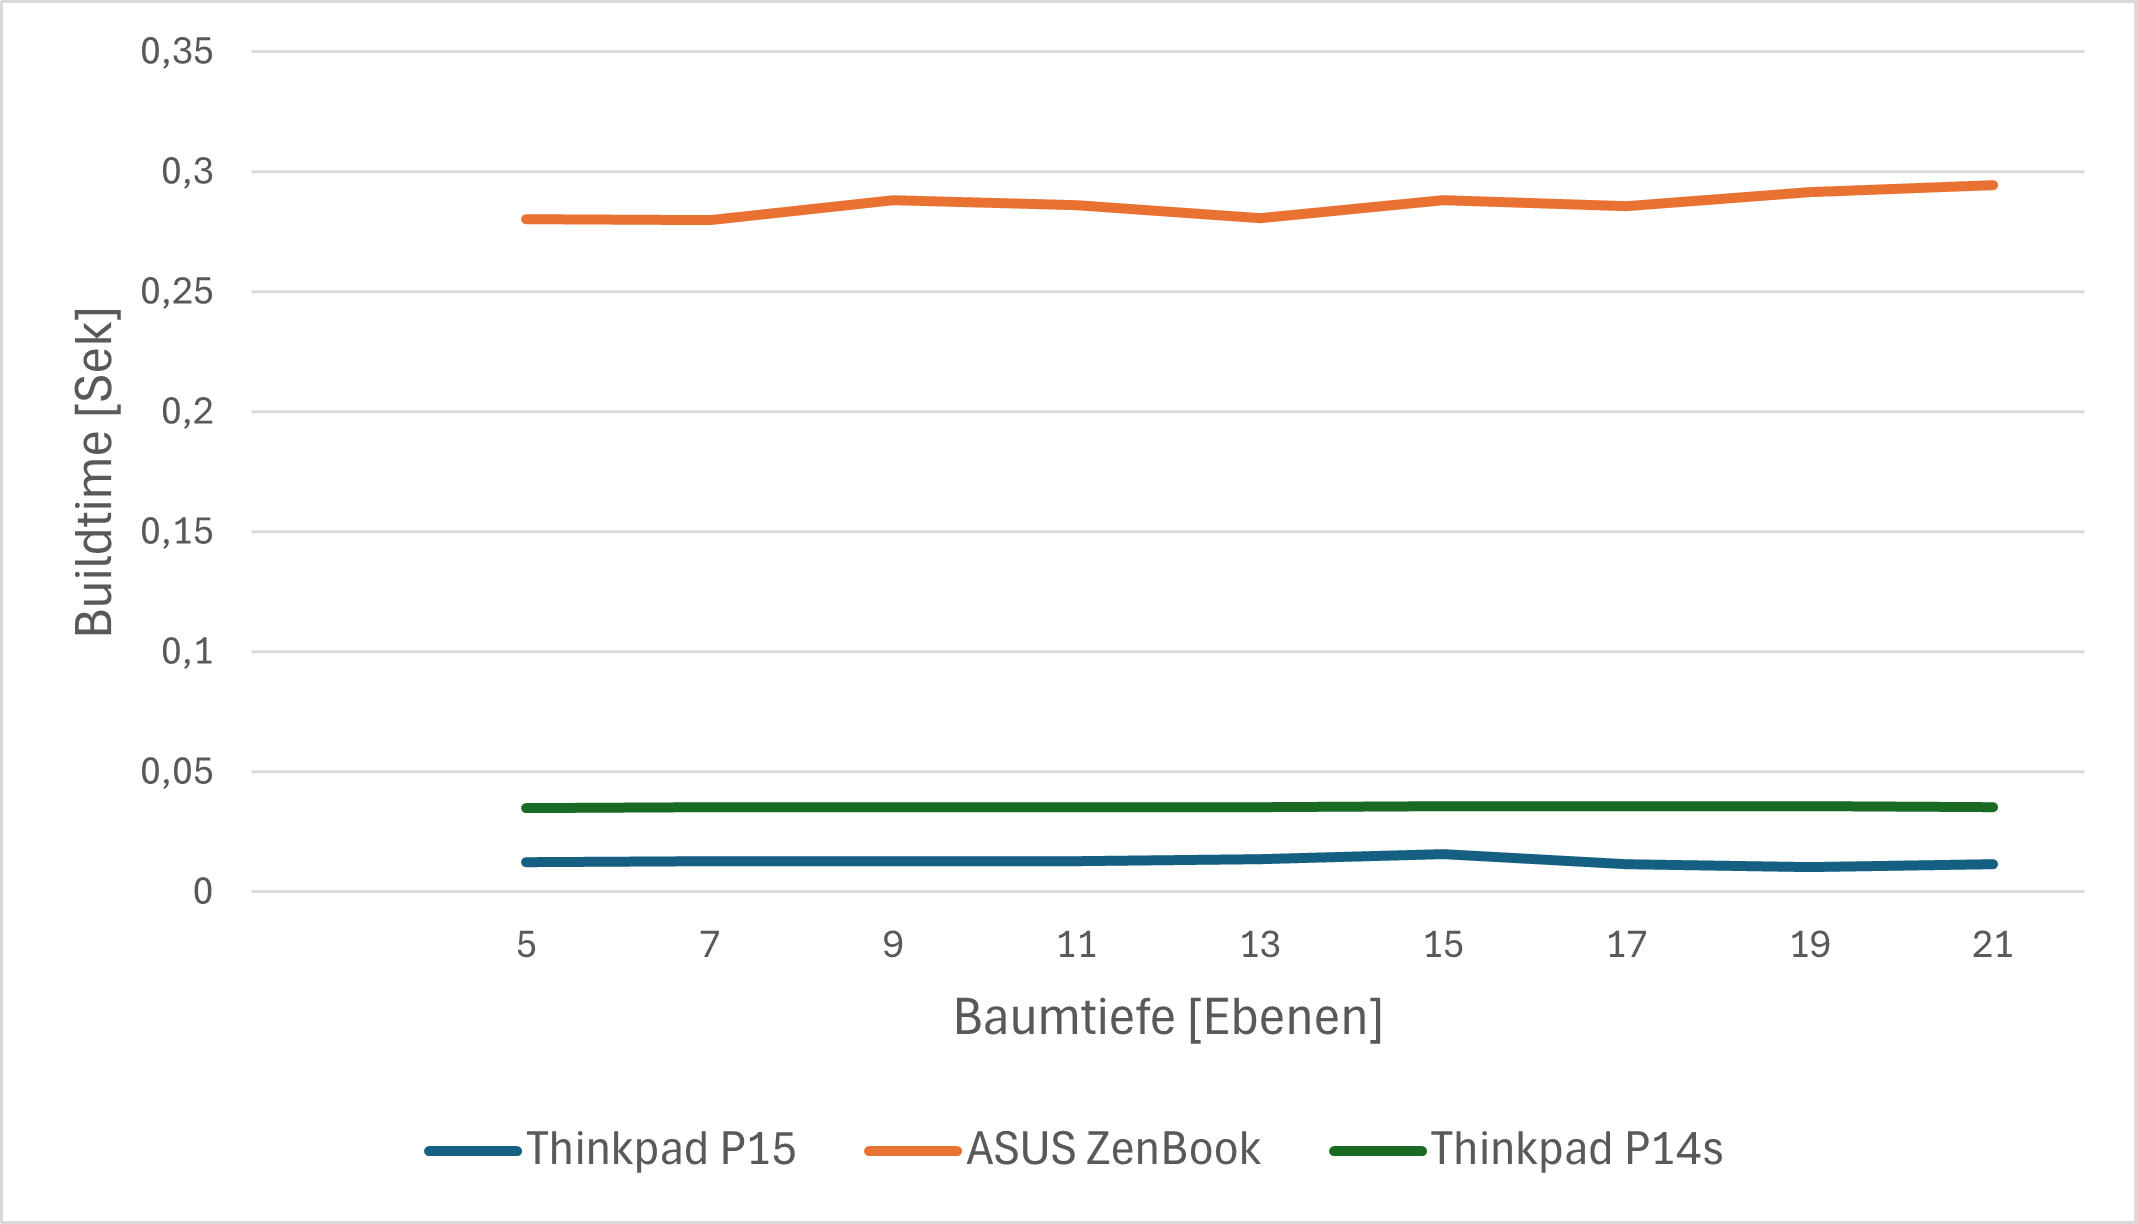
\includegraphics[width=\linewidth]{diagrams/OpenCL_Buildtime.png}
    \captionof{figure}{Buildzeit OpenCL-Kerlen auf verschiedenen Rechnern}
\end{minipage}
\hfill
\begin{minipage}{0.49\linewidth}
    Ein wichtiger Einflussfaktor auf die Laufzeit von OpenCL ist die Zeit, die für den Kernel-Bau vonnöten ist. 
    Die obigen Diagramme zeigen die Ausführungszeit bereits kompilierten Codes. 
    Wie das Diagramm links abbildet, ist die Buildtime weitgehend unabhängig von der Baumtiefe, variiert jedoch je nach 
    Rechner --- auf schnellen Systemen liegt sie unter 0,015 Sekunden, auf langsameren unter 0,3 Sekunden. 
\end{minipage} 

% ----------------------------------- Auslastung CPU / Speicher -----------------------------------
% -------------------------------------------------------------------------------------------------
\vspace{0.25cm}
\subsection{Auslastung von CPU und Speicher}\label{Speicher}
\vspace{-0.25cm}
Um sicherzustellen, dass --- besonders bei der parallelen Implementierung mit OpenMP --- die CPU tatsächlich 
ausgelastet wird, haben wir die Auslastung der CPU und des Speichers während der Programmausführung überwacht.

\begin{figure}[!ht]
    \centering
    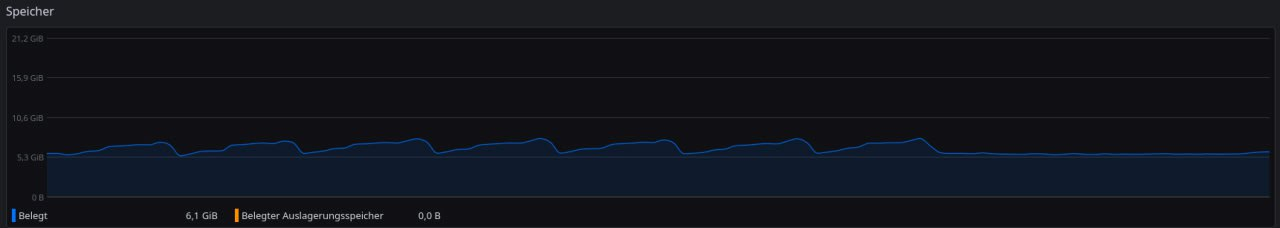
\includegraphics[width=\linewidth]{./diagrams/Memory.jpg}
    \caption{Auslastung des RAM eines Thinkpad P14s Gen 1 während der Programmausführung}
    \label{fig:memory}
\end{figure}
\vspace{-0.25cm}
\noindent Grafik~\ref{fig:memory} zeigt die RAM-Auslastung eines Thinkpad P14s Gen 1 während eines Programmlaufs. 
Dabei entspricht ein Intervall der Kurve, in welchem der Graph bis zu einem Hochpunkt steigt und anschließend auf 
einen Tiefpunkt abfällt, einer Programmausführung.\\
Die Auslastung des RAMs war bei allen Arten der Implementierung (seriell iterativ, parallel mit OpenMP, parallel 
mit OpenCL) sehr ähnlich.

\vspace{0.5cm}
\begin{figure}[!ht]
    \centering
    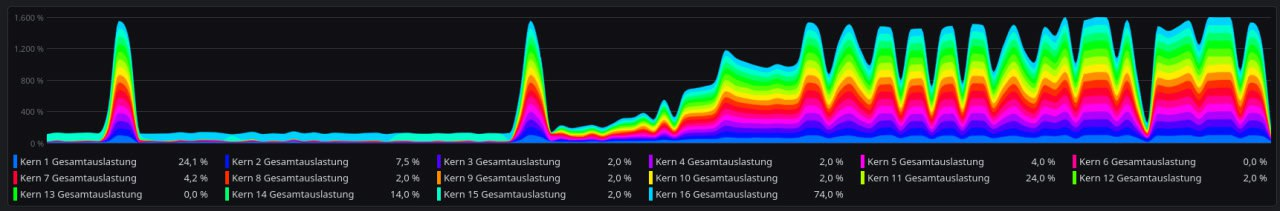
\includegraphics[width=\linewidth]{./diagrams/Serial-OpenMP.jpg}
    \caption{CPU-Auslastung im Übergang von sequentieller zu paralleler Berechnung mit OpenMP}
    \label{fig:Serial-OpenMP}
\end{figure}
\vspace{-0.25cm}
\noindent In Grafik~\ref{fig:Serial-OpenMP} ist die CPU-Auslastung während eines Programmlaufs mit anfangs sequentieller 
und später CPU-paralleler Ausführung zu sehen.\\
Die einzelnen Hochpunkte des Graphen in der ersten Hälfte des Diagrams kommen zustande, weil das Hinzufügen der
Quadern zum Renderer mit OpenMP parallelisiert erfolgt, um eine optimale Ausführungszeit gewährleisten zu können.
Die entsprechende Funktion \texttt{addRenderObject()} ist im Renderer angesiedelt und für alle unsere Implementierungen 
gleich.\\
Zu sehen ist auch, dass erst bei späten Baumtiefen eine Auslastung mehrerer Kerne erreicht wird. 

\vspace{0.5cm}
\begin{figure}[!ht]
    \centering
    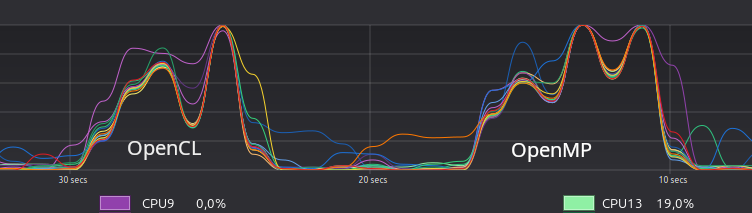
\includegraphics[width=0.9\linewidth]{./diagrams/OpenCL-OpenMP.png}
    \caption{CPU-Auslastung OpenCL im Vergleich zu OpenMP}
    \label{fig:CPU-OpenCL-OpenMP}
\end{figure}
\vspace{-0.25cm}
\noindent
Wie Grafik~\ref{fig:CPU-OpenCL-OpenMP} zeigt, ist die CPU-Auslastung bei einer parallelisierten Ausführung mit 
einer Baumtiefe von 21 Ebenen bei OpenCL minimal geringer als bei OpenMP --- jedoch deutlich weniger, als zu erwarten war. 
Dies ist damit zu begründen, dass die Berechnung der Quader auf der GPU erfolgt, das Übertragen der Daten an den
Renderer aber auf der CPU stattfindet. Während diese Weiterverarbeitung der generierten Daten in der seriellen Implementierung bis 
auf die letzte Ebene seriell ausgeführt wird, ist sie bei der OpenCL-Implementierung mit OpenMP parallelisiert, um eine Verunreinigung
der Zeitmessungen durch den Renderer möglichst gering zu halten. Einen nicht zu vernachlässigenden Rechenaufwand stellt dabei das 
Überführen der von der GPU zurückgelieferten Werte in ein vom Renderer anzeigbares Format.\\

\vspace{0.5cm}
\begin{figure}[!ht]
    \centering
    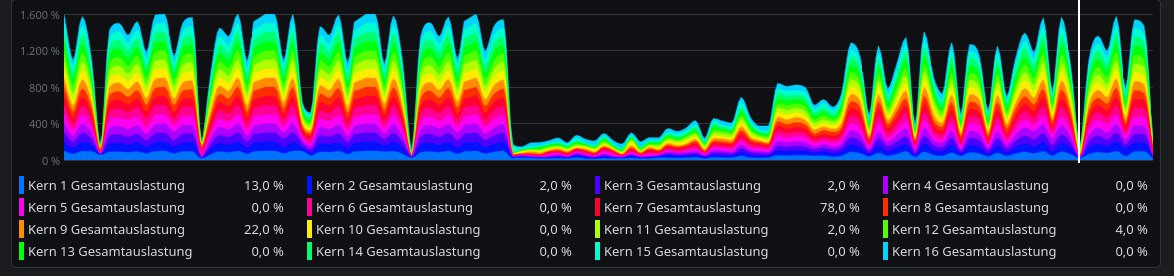
\includegraphics[width=0.9\linewidth]{./diagrams/OpenMP-OpenCL-POCL.jpg}
    \caption{CPU-Auslastung bei paralleler Programmausführung mit Übergang von OpenMP zu OpenCL}
    \label{fig:OpenMP-OpenCL}
\end{figure}

\noindent
Grafik \ref{fig:OpenMP-OpenCL} bildet die CPU-Auslastung während eines parallelen Programmablaufs ab, bei welchem 
zuerst mit OpenMP und danach mit OpenCL gearbeitet wird. Wie gut zu erkennen ist, ist die CPU-Auslastung für große Baumtiefen während beider Ausführungen bei allen Kernen 
vergleichsweise hoch, was darauf zurückzuführen ist, dass aus \hyperref[Hardware]{hardwaretechnischen Gründen} auch die OpenCL-Implementierung
auf der CPU ausgeführt wird.\\
Interessant ist, dass in diesem Fall die CPU-Auslastung mit OpenCL augenscheinlich geringer war, während die Laufzeit dennoch niedriger
blieb. Der Abschnitt hinter der in der Grafik eingezeichneten weißen Linie zeigt eine Ausführung des Programms mit 21 Ebenen unter 
Verwendung von OpenCL, also ebenso wie die letzten Ausführungen unter Verwendung von OpenMP. \\

% ----------------------------------- Beschleunigung (Amdahl) -----------------------------------
% -----------------------------------------------------------------------------------------------
\subsection{Beschleunigungsfaktor nach Amdahl}
\flushleft Zur Bestimmung des Beschleunigungsfaktors nach Amdahl erfassten wir einmalig die serielle Ausführungszeit (SERT) und 
gleichzeitig die Laufzeit des parallelisierbaren Codes (PT). Aus diesen \hyperref[Anhang]{Messwerten} berechneten wir die benötigten Parameter
\vspace{0.15cm}\\
\centering $P = PT / SERT$ und $S = (SERT - PT) / SERT$ 
\vspace{-0.15cm}
\flushleft sodass wir letztendlich für die verschiedenen Baumtiefen die Beschleunigungsfaktoren kalkulieren konnten:
\begin{table}[H]
    \centering
    \small
    \begin{tabular}{@{}cccccc@{}}
        \toprule
        Baumtiefe & P        & N    & S         & Beschleunigungsfaktor \\ \midrule
        1         & 0.333   & 4096 & 1.000     & 1.500 \\
        2         & 0.000   & 4096 & 0.667     & 1.000 \\
        3         & 0.000   & 4096 & 3.334     & 5.999 \\
        4         & 0.286   & 4096 & 0.714     & 5.993 \\
        5         & 0.000   & 4096 & 4.286     & 7.190 \\
        6         & 0.913   & 4096 & 0.728     & 3.999 \\
        7         & 0.000   & 4096 & 5.000     & 8.524 \\
        8         & 0.000   & 4096 & 2.157     & 3.037 \\
        9         & 0.000   & 4096 & 6.205     & 9.867 \\
        10        & 0.995   & 4096 & 0.722     & 5.156 \\
        11        & 0.895   & 4096 & 0.712     & 5.966 \\
        12        & 0.835   & 4096 & 0.361     & 3.021 \\
        13        & 0.892   & 4096 & 0.719     & 6.234 \\
        14        & 0.899   & 4096 & 0.861     & 6.635 \\
        15        & 0.821   & 4096 & 0.814     & 6.996 \\
        16        & 0.000   & 4096 & 8.575     & 12.756 \\
        17        & 0.000   & 4096 & 0.686     & 5.581 \\
        18        & 0.000   & 4096 & 0.838     & 7.648 \\
        19        & 0.055   & 4096 & 1.116     & 10.553 \\
        20        & 0.000   & 4096 & 0.190     & 3.803 \\
        21        & 0.811   & 4096 & 0.190     & 5.275 \\ \bottomrule
    \end{tabular}
    \caption{Beschleunigungsfaktor nach Amdahl für verschiedene Baumtiefen}
\end{table}

Entgegen unserer auf den zuvor aufgeführten Laufzeitanalysen basierenden Erwartungen zeigte sich anhand der ermittelten Werte
keine deutliche Verbesserung der Beschleunigung mit höheren Baumtiefen. Stattdessen unterlag der Wert massiven Schwankungen. 
Nichtsdestotrotz spiegelt sich auch im folgend beigefügten Diagramm ein Anstieg der Beschleunigung im Vergleich von hohen
zu niedrigen Baumtiefen wider.\\
Der höchste feststellbare Beschleunigungsfaktor lag zwischen 18 und 19. Diesen bestimmten wir, indem wir zuerst in unserer Tabelle 
mit den Beschleunigungen für die verschiedenen Baumtiefen durch das Testen steigender Werte für N (Anzahl GPU-Cores) den Baum mit 
Tiefe neun als den mit der größten Beschleunigung feststellten. Danach bestimmten wir den Grenzwert der monoton steigenden, nach oben
beschränkten Kurve, welche die Beschleunigung bei einer Tiefe von neun Ebenen für eine steigende Anzahl GPU-Cores abbildet.
\vspace{0.5cm}\\
\begin{minipage}{0.49\linewidth}
    \centering
    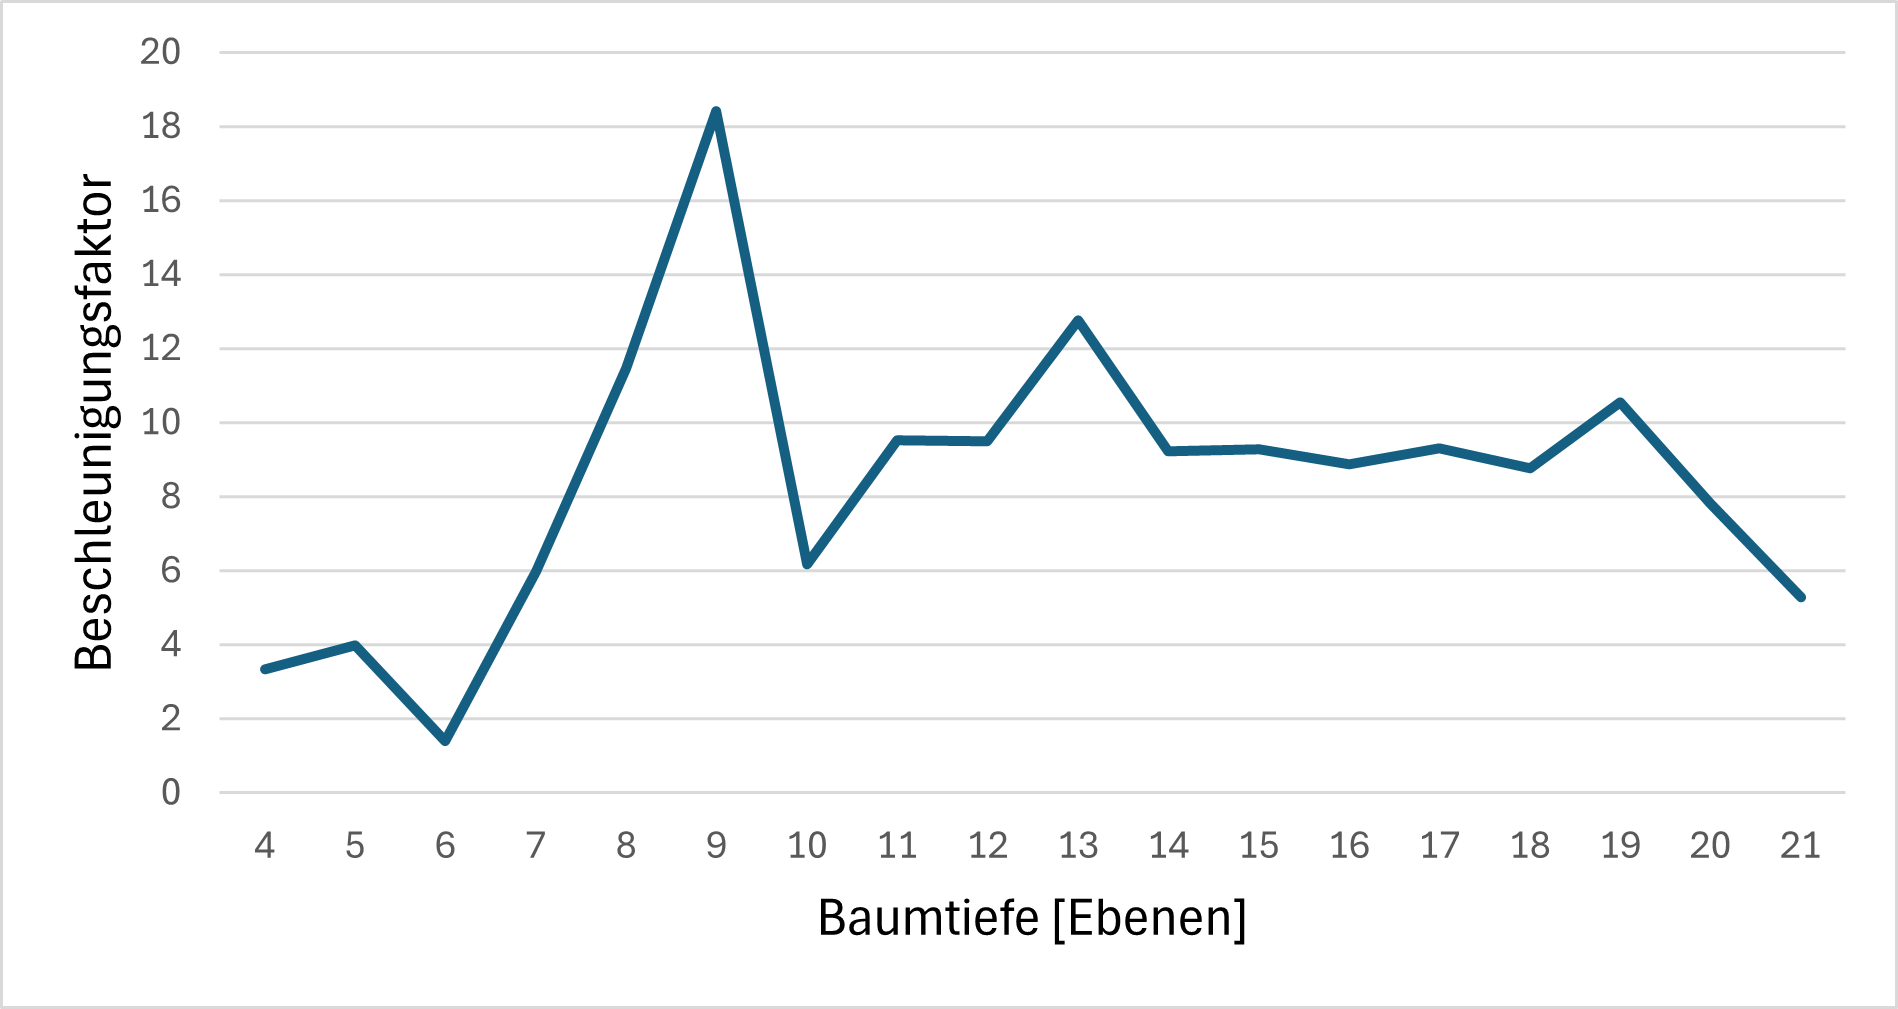
\includegraphics[width=\linewidth]{diagrams/Amdahl_Nvidia4096.png}
    \captionof{figure}{Beschleunigung nach Amdahl für verschiedene Baumtiefen auf Nvidia RTX A3000 mit 4096 Cores}
    \label{fig:AmdahlsLaw}
\end{minipage}
\hfill
\begin{minipage}{0.49\linewidth}
    \centering
    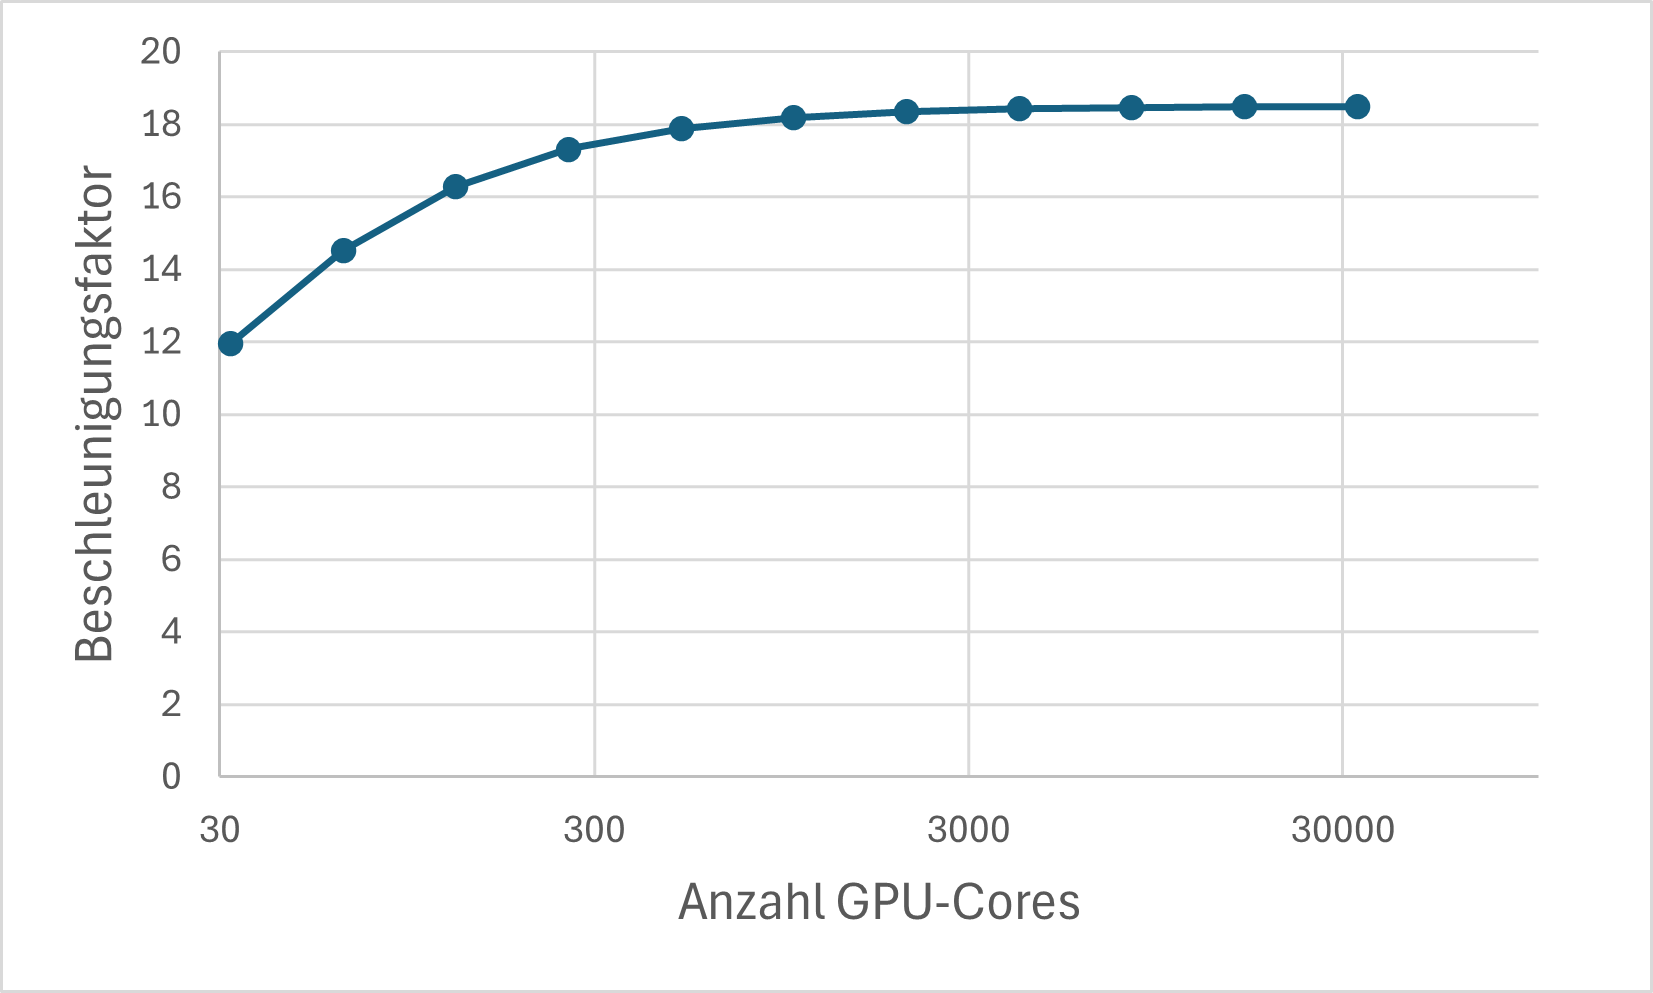
\includegraphics[width=\linewidth]{diagrams/Amdahl_maxBeschleunigung.png}
    \captionof{figure}{maximale Beschleunigung nach Amdahl auf Nvidia RTX A3000}
    \label{fig:AmdahlMaxBeschleunigung}
\end{minipage}

% ----------------------------------- Ansätze kombinieren ---------------------------------------
% -----------------------------------------------------------------------------------------------
\vspace{0.25cm}
\subsection{Kombinieren verschiedener Ansätze}\label{openCL-Fehler}
\vspace{-0.25cm}
Die mit den Ebenen steigende Komplexität unseres Programms hat einen großen Einfluss auf 
seine Gesamtlaufzeit. Für die ersten Ebenen bringen Parallelisierungen einen großen Overhead
mit sich, bei späteren Ebenen sind sie jedoch wesentlich schneller als die sequentielle Ausführung.\\
Zum Erreichen einer möglichst guten Programmlaufzeit entschlossen wir uns, die einzelnen 
Technologien kombiniert auszuführen. An welchen Stellen optimalerweise zwischen den Ansätzen
gewechselt werden sollte, ließ sich dabei gut aus den Schnittpunkten in den Laufzeit-Graphen ableiten. 
Diese sind zwar für jedes Endgerät unterschiedlich, können aber anhand unserer Erkenntnisse grob festgelegt werden.
\\Auf dem Thinkpad P15 konnten wir folgende Ergebnisse erzielen:
\begin{itemize}[itemsep=0pt, parsep=0pt, topsep=0pt, partopsep=0pt]
    \item Baum der Tiefe 24: ca. 17 Sekunden\\
            Ebenenverteilung: seriell 7 / OMP 16 / OCL 1 Ebenen
    \item Baum der Tiefe 24: ca. 10 Sekunden\\
            Ebenenverteilung: seriell 9 / OMP 15 Ebenen
    \item Baum der Tiefe 25: ca. 45 Sekunden\\
            Ebenenverteilung: seriell 9 / OMP 14 / OCL 2 Ebenen
\end{itemize}
Auf einem Desktop-PC wurden 24 Ebenen mit einer Verteilung von seriell 5 Ebenen, OpenMP 12 Ebenen und 
OpenCL 6 Ebenen als bestmögliche Baumtiefe in kürzestmöglicher Zeit  erreicht.
\vspace{0.25cm}\\
Im Rahmen unserer Analysen stießen wir auf zwei verschiedene Bottlenecks, welche beide an die Speicherkapazität
gebunden sind: 
Wie im folgenden Abschnitt \hyperref[Speicher]{5 Speicher} ausführlich evaluiert, wächst der Speicherplatzbedarf
für die Quader quadratisch. Daraus resultiert, dass Bäume mit mehr als 23 Ebenen in der Regel nicht generierbar sind.\\
Weiterhin tritt sofern man OpenCL mit großen Tiefen ausführt je nach Rechner zu unterschiedlichen Zeitpunkten 
der Fehlercode \texttt{-4 CL\_MEM\_OBJECT\_ALLOCATION\_FAILURE} auf, welcher auf nicht genügend verfügbaren Speicher
auf der GPU hindeutet. Diesen erhielten wir auf dem Thinkpad P15 ab der 26. Ebene und auf dem Thinkpad P14s ab der 24. Ebene. 

\newpage
\section{Speicher}
\vspace{-0.25cm}
\subsection{Speicherverbrauch}
\vspace{-0.25cm}
Ein essentieller Punkt in Bezug auf die maximal mögliche Baumtiefe in unserem Programm ist der Speicherverbrauch.
Maßgeblich ist hier das Array, in welchem die generierten Quader (Datentyp Cuboid) gespeichert werden. 
Die Größe eines Cuboids setzt sich wie folgt zusammen:
\vspace{0.25cm}\\
\begin{minipage}{0.4\linewidth}
    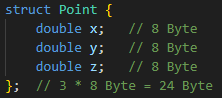
\includegraphics[width=\linewidth]{./pictures/SpeicherverbrauchPoint.PNG}
\end{minipage}
\hfill
\begin{minipage}{0.58\linewidth}
    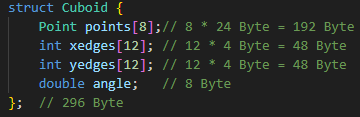
\includegraphics[width=\linewidth]{./pictures/SpeicherverbrauchCuboid.PNG}
\end{minipage}
\vspace{0.5cm}\\
Um die Daten sinnvoll im Speicher platzieren zu können, fügt der Compiler gegebenenfalls noch 8 Byte Padding pro Cuboid hinzu. 
Der Speicherplatzbedarf pro Quader liegt also bei 296 Byte oder 304 Byte. 
\vspace{0.5cm}\\
\begin{minipage}{0.55\linewidth}
    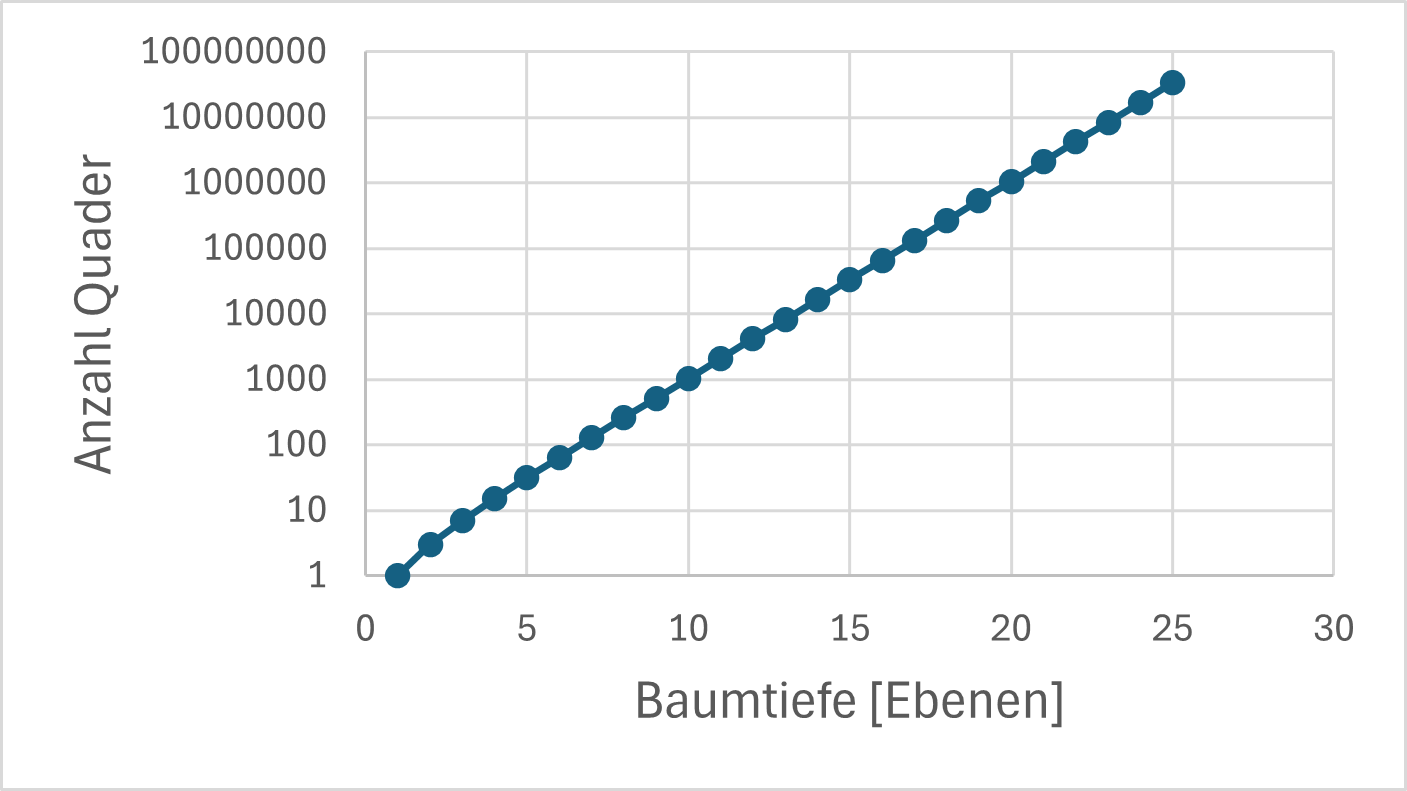
\includegraphics[width=\linewidth]{./diagrams/CuboidsProEbene.png}
    \captionof{figure}{Gesamtanzahl Quader pro Baumtiefe}
    \label{fig:CuboidsProEbene}
\end{minipage}
\hfill
\begin{minipage}{0.43\linewidth}
    Für jeden Quader in der aktuellen Ebene sind in der darauffolgenden Ebene zwei neue Quader zu generieren.
    Die Anzahl der zu generierenden Quader des Baums steigt also quadratisch mit der Funktion
    \vspace{-0.25cm} \center{$f(n) = 2^n - 1$,} \\
    wobei $n$ die Anzahl der Ebenen im Baum ist.
\end{minipage}
\vspace{0.5cm}

\noindent
\begin{minipage}{0.39\linewidth}
    Daraus ergibt sich, dass der benötigte Speicherplatz allein für die Quader ab einer Baumtiefe von 
21 Ebenen > 1 GB ist. Für 25 Ebenen werden annähernd 20 GB benötigt.
\end{minipage}
\hfill
\begin{minipage}{0.56\linewidth}
    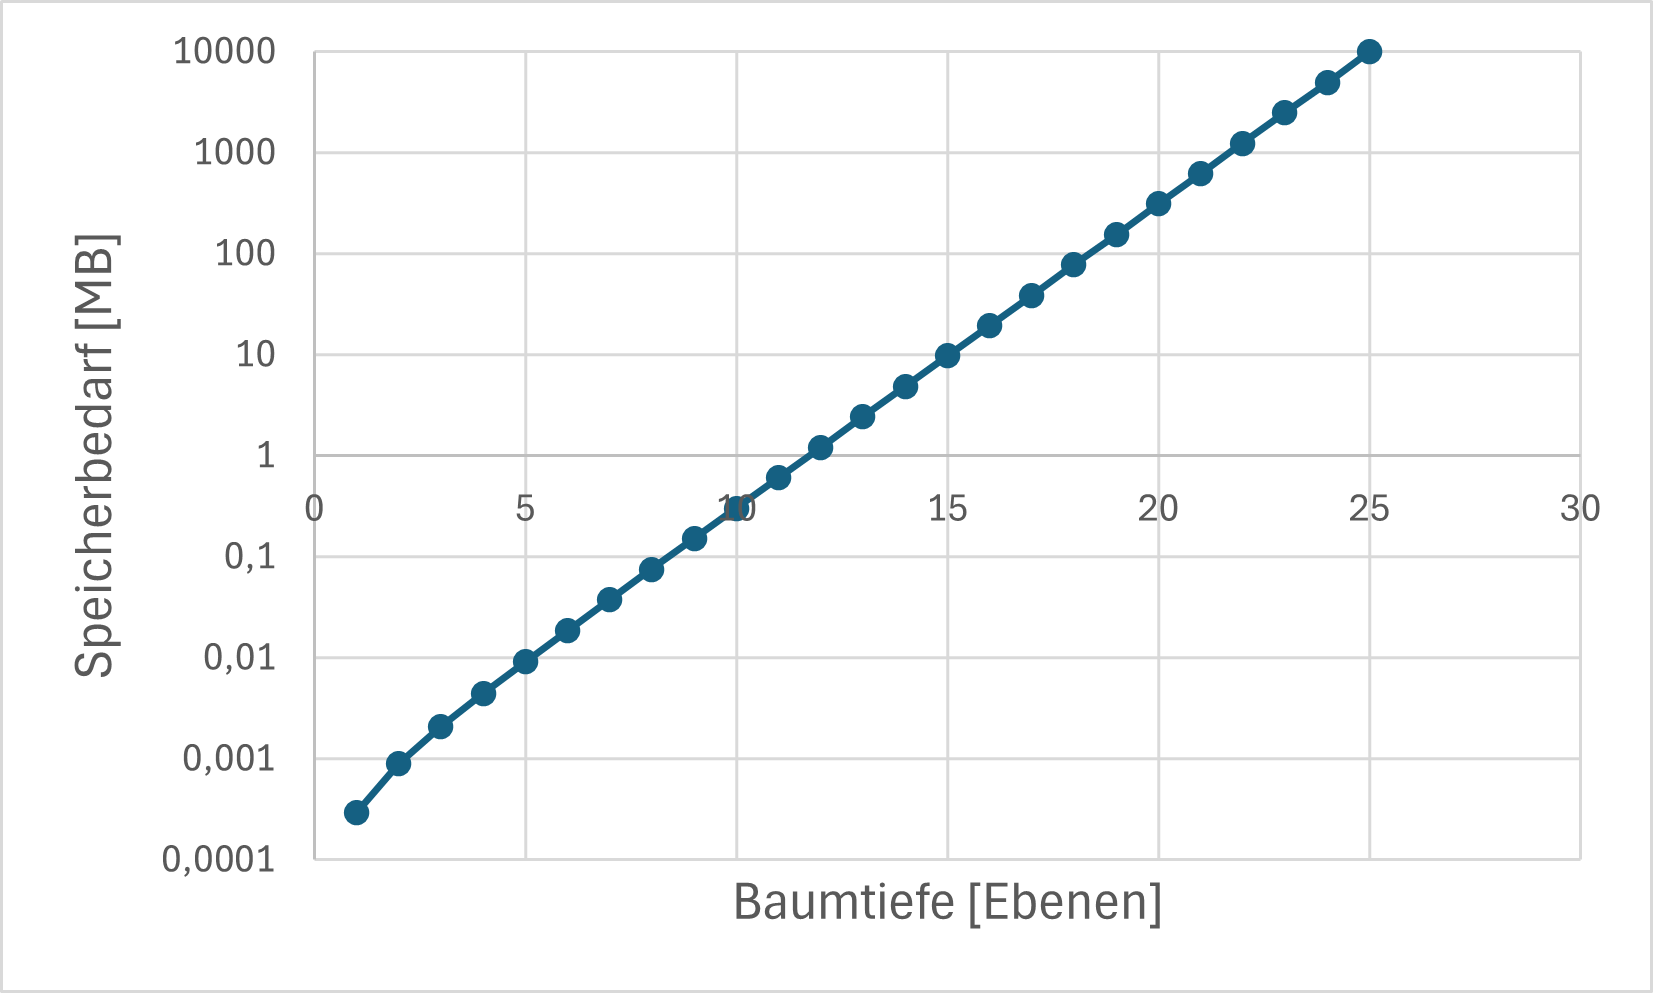
\includegraphics[width=\linewidth]{./diagrams/Speicherplatzbedarf.png}
    \captionof{figure}{Gesamtspeicherbedarf Quader in Megabyte}
\end{minipage}
\vspace{0.5cm}\\
Dementsprechend ist der ausschlaggebende Faktor für die maximale Baumtiefe nicht etwa die Schnelligkeit 
des Prozessors oder der GPU, sondern der im RAM verfügbare Speicherplatz. 

\newpage
\subsection{Einfluss der Speicherhierarchie}
\vspace{-0.25cm}
Da die Quader jeder Ebene in einem Array (bzw. Vector) gespeichert werden, sind ihre Daten in einem 
zusammenhängenden Bereich im Hauptspeicher abgelegt.\\
Bei OpenMP wird direkt über dieses Array iteriert, weshalb die Zugriffszeit auf die Daten durch Caching stark 
reduziert werden kann. Im Vergleich dazu wäre der Einsatz einer Verkettete Liste für die gleiche Aufgabe
deutlich langsamer.\\
Bei OpenCL müssen die Daten jedes Mal von der CPU auf die GPU und zurück übertragen werden. Dadurch spielt der Cache
hier eine untergeordnete Rolle. Allerdings müssen die Daten nichtsdestotrotz in einem zusammenhängenden Block abgelegt sein, 
weil für die Erzeugung der Buffer ein Zeiger auf den zu kopierenden Speicherbereich benötigt wird. Dies ermöglicht
vermutlich eine Art DMA über PCIe. Eine Beschleuningung des Programmanblaufs durch Caching ist im mit OpenCL parallelisierten
Bereich deshalb nur bei der Übertragung von Werten in den Renderer möglich. Diese erfolgt wiederum durch eine mit OpenMP
paralleliserte Schleife, die über einen zusammenhängenden Speicher (Vector) iteriert.

  

\newpage
\section{Weitere Verbesserungen}
\vspace{-0.25cm}
Im Laufe unserer Projektumsetzung stießen wir an einigen Stellen auf Probleme, deren Beseitigung den zeitlichen Rahmen gesprengt hätte.
Dennoch gab es eine Reihe von Ideen für mögliche Lösungen, auf welche wir im folgenden kurz eingehen: 

\vspace{-0.25cm}
\subsubsection*{Synchronisaton}
\vspace{-0.25cm}
Wie in \hyperref[3-2-rendering]{Abschnitt 3.2 Hinzufügen von Objekten zum Renderer} beschrieben, verwenden wir derzeit einen kritischen Bereich,
um das Hinzufügen von Quadern zum Renderer fehlerfrei zu ermöglichen. Über ein Array vordefinierter Größe im Renderer sollte es möglich
sein, diese Operation mit Hilfe der Thread-IDs zu parallelisieren. 

\subsection*{OpenCL}
\vspace{-0.25cm}
\subsubsection*{Speicherverbrauch}
\vspace{-0.25cm}
Ein zentrales Problem der aktuellen OpenCL-Variante ist der Speicherbedarf auf dem Device. Für größere Baumtiefen übersteigt die benötigte Buffergröße den auf der GPU
verfügbaren Speicherplatz, sodass OpenCL mit \texttt{CL\_MEM\_OBJECT\_ALLOCATION\_FAILURE (-4)} abbricht (vgl. \hyperref[openCL-Fehler]{Abschnitt 4.6})\\
Eine Verbesserung könnte durch aufsplitten der Transfers bzw. Speicherobjekte erreicht werden. Statt für eine komplette Ebene einen großen 
Eingabe- und Ausgabebuffer zu reservieren, könnte die Ebene in mehrere Pakete zerlegt werden, die nacheinander verarbeitet werden. 
Dadurch sinkt die maximal benötigte Buffergröße und damit die Wahrscheinlichkeit, dass Allokationen aufgrund fragmentierten oder zu
knappen Device-Speichers fehlschlagen.

\vspace{-0.25cm}
\subsubsection*{Optimierung der Blockgröße und -anzahl}
\vspace{-0.25cm}
Die Optimierung von Blockgröße und Blockanzahl erwies sich als schwierig. Der Hauptgrund ist, dass sich die Anzahl der zu verarbeitenden
Quader pro Ebene verdoppelt, wodurch sich die optimale Verteilung stetig verändert.\\
Als Ansatz zur Verbesserung bietet sich hier eine Pipelinestruktur an. Die Grundidee ist, fortlaufend Pakete von Quadern zu verarbeiten:
Die CPU schickt ein Paket von Quadern an die GPU.
Die GPU erzeugt daraus die neuen Quader (Folgeebene) und schreibt sie in einen Ausgabebuffer.
Während die GPU bereits am nächsten Paket arbeitet, holt die CPU die Ergebnisse des vorherigen Pakets ab --- parallel dazu kann die CPU den Renderer 
befüllen und die bereits generierten Quader zur Darstellung weiterreichen.\\
So entsteht eine Überlappung von Rechenzeit und Transfer-/Verarbeitungszeit, weil die CPU den Renderer befüllt, während die GPU arbeitet.
Im Idealfall reduziert dies Wartezeiten und steigert den Durchsatz des Systems. \\
Ein praktischer Nebeneffekt wäre, dass die Blockgröße durch die Paketgröße automatisch beschränkt würde, was nicht nur die Wahl passender Work-Group-Größen
erleichtert, sondern auch das zuvor beschrieben Problem mit den Speicherlimits reduzieren könnte.

\newpage
\subsection*{Renderer}
Obwohl wir vor allem mit den parallelen Ansätzen theoretisch recht große Bäume generieren können, ist es uns praktisch derzeit nicht möglich, diese
visuell aufzubereiten. Außerdem wäre in Anlehnung an den Fraktal-Charakter der Pythagorasbäume eine Zoom-Option im Renderer von Vorteil.\\
Um die Effizienz unseres Renderers zu verbessern, böte sich Multithreading oder die Verwendung von Hardwarebeschleunigung an. 


\newpage
\section{Fazit}
Im Rahmen dieser Arbeit konnten wir zeigen, dass sich die Erzeugung eines 3D Pythagoras-Baums gut als datenparalleles Problem
modellieren lässt, da zwischen den Quadern keine Abhängigkeiten bestehen und somit kaum Synchronisation nötig ist. Entscheidend 
für die erfolgreiche Parallelisierung war die Umstellung von einer rekursiven auf eine iterative, ebenenweise Berechnung, weil sich 
nur so die Arbeit sinnvoll auf CPU-Kerne bzw. GPU-Threads verteilen lässt.\\
Unsere Laufzeitanalyse zeigte, dass der Overhead paralleler Ansätze für kleine Baumtiefen (insbesondere bei OpenCL durch 
Speichertransfer und Kernel-Setup) sehr groß ist, während bei größeren Tiefen deutliche Zeitgewinne möglich sind. OpenMP erwies 
sich als überaus nützlich, während OpenCL zwar bei großen Tiefen Vorteile bringen kann, jedoch stark von 
Hardware/Implementierung abhängt (z. B. PoCL-Effekt durch Wegfall des GPU-Transfers).\\
Der zentrale limitierende Faktor unseres Projekts ist nicht die Rechenleistung, sondern der Speicher. Bereits ab ca. 21 Ebenen
liegt der Bedarf allein für die Quaderdaten im Gigabyte-Bereich, bei 25 Ebenen im zweistelligen Gigabyte-Bereich.
Deshalb waren Bäume mit mehr als ca. 23 Ebenen in der Praxis nicht mehr wirklich generierbar.\\
Als naheliegende Weiterentwicklungen bieten sich insbesondere eine Pipeline-/Paketierung der OpenCL-Transfers, das Reduzieren 
verbleibender kritischer Bereiche sowie eine stärkere Parallelisierung bzw. Beschleunigung des Renderers an.

\newpage
\section{Nobody is perfect}
\begin{figure}[H]
    \centering
    
\includegraphics[width=0.98\linewidth]{pictures/outtakes/Outtakes.png}
\end{figure}
\vfill
% Anhang
\section*{Anhang}\label{Anhang}
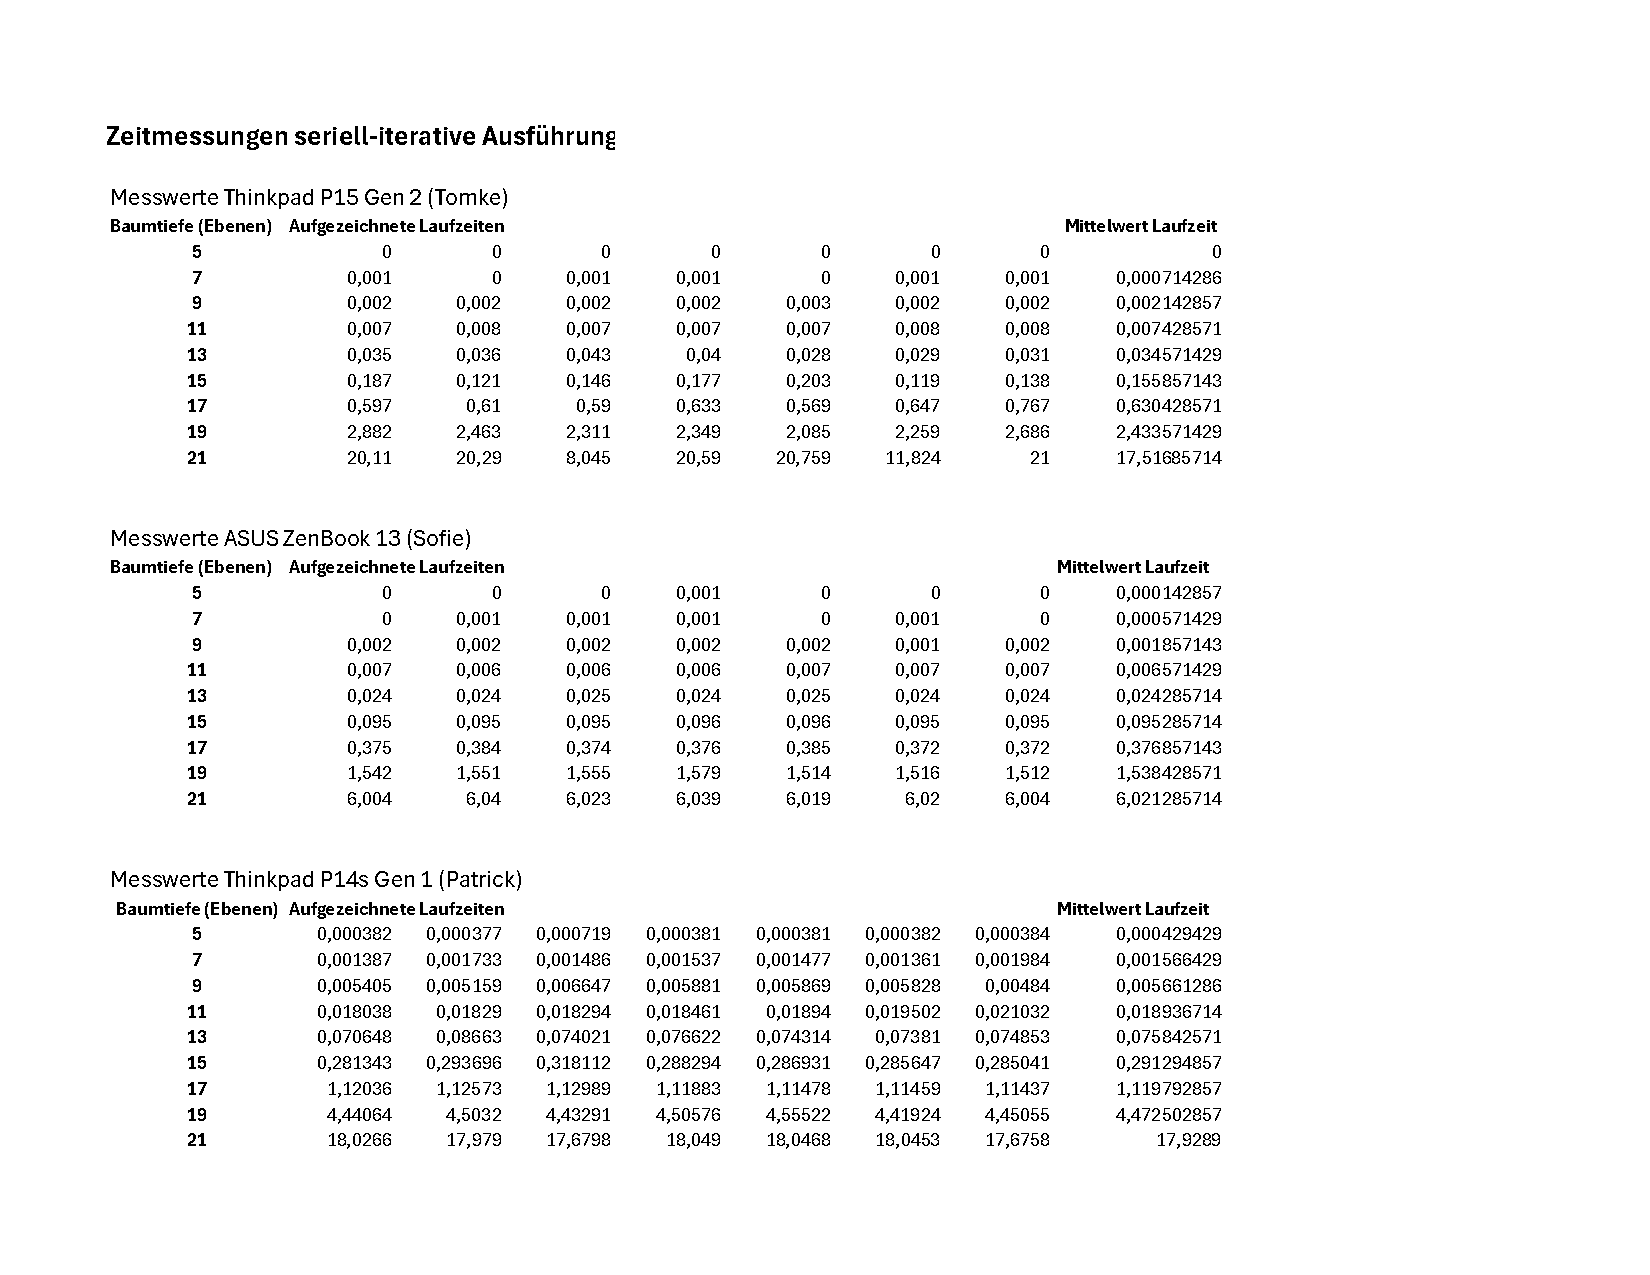
\includepdf[pages=-, fitpaper=true]{appendix/Zeiten_seriell.pdf}
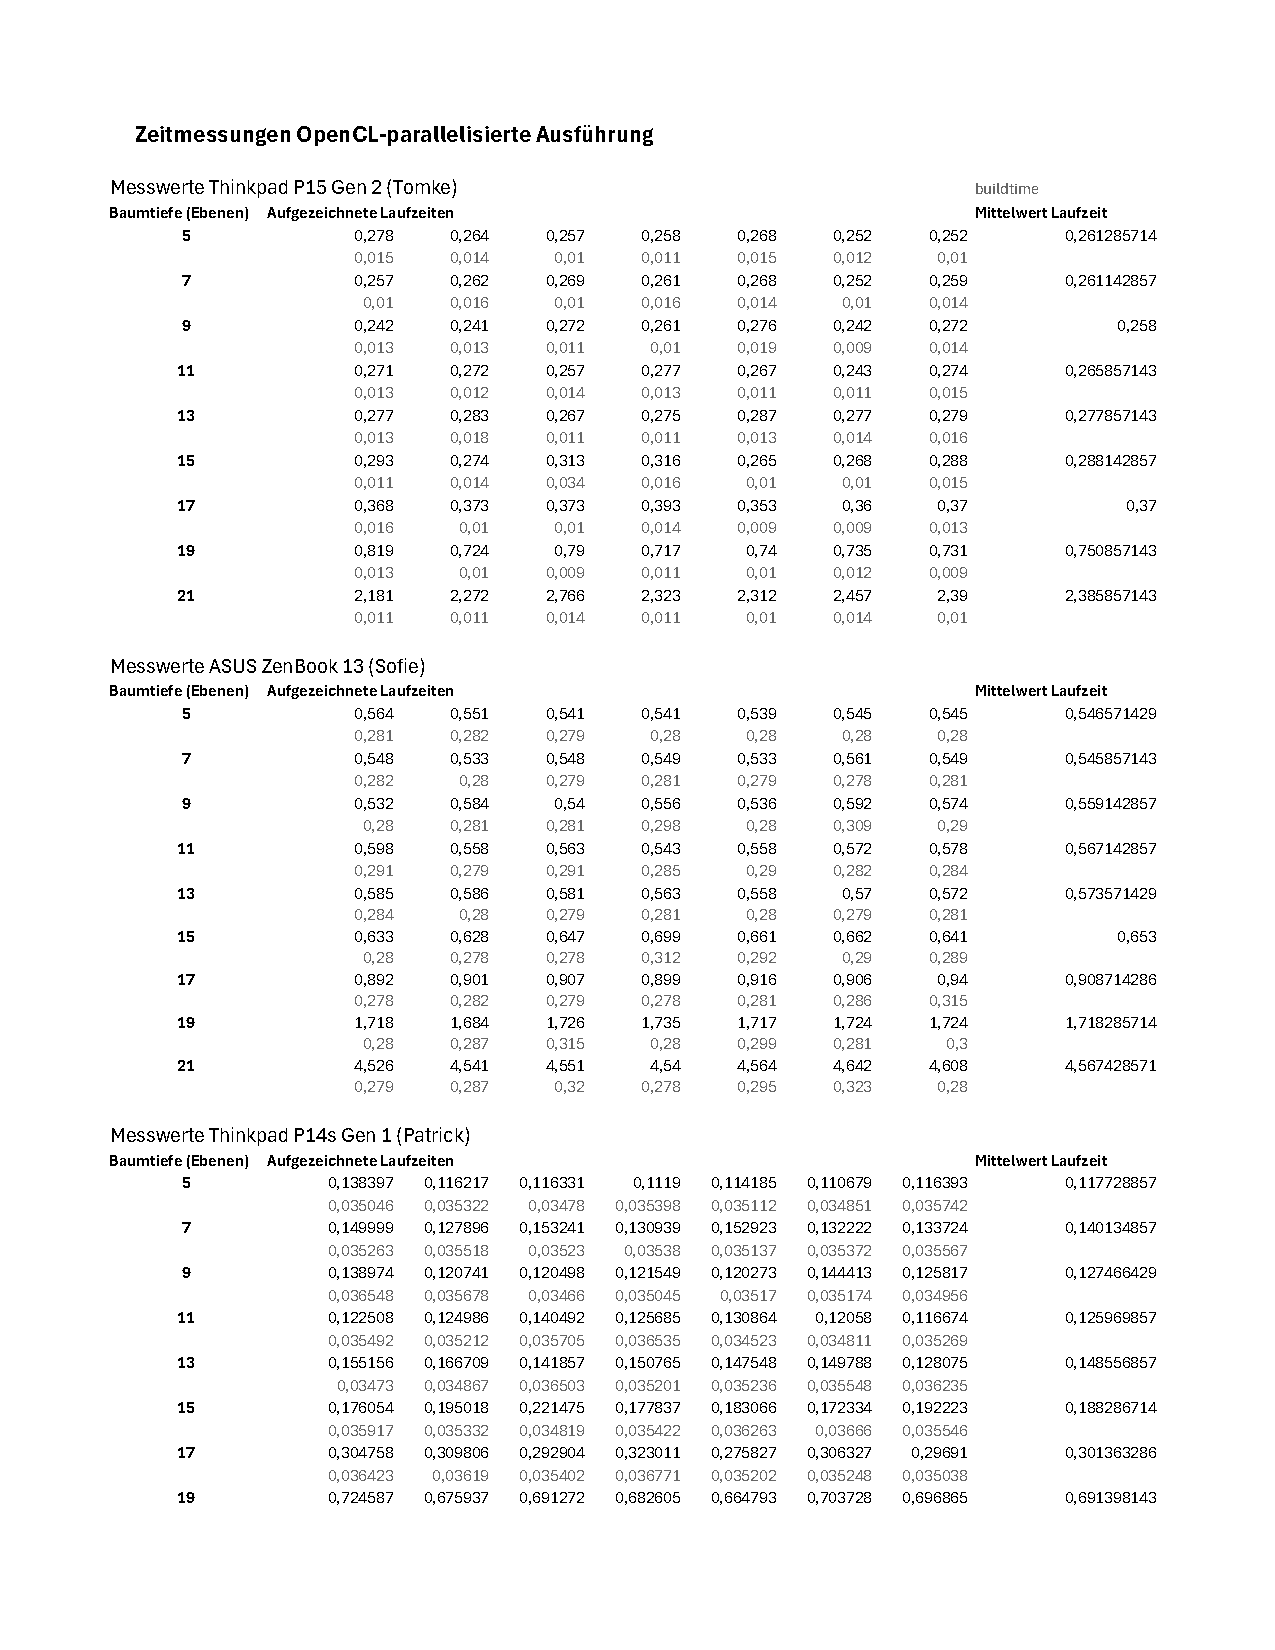
\includepdf[pages=-, fitpaper=true]{appendix/Zeiten_parallel_ocl.pdf}
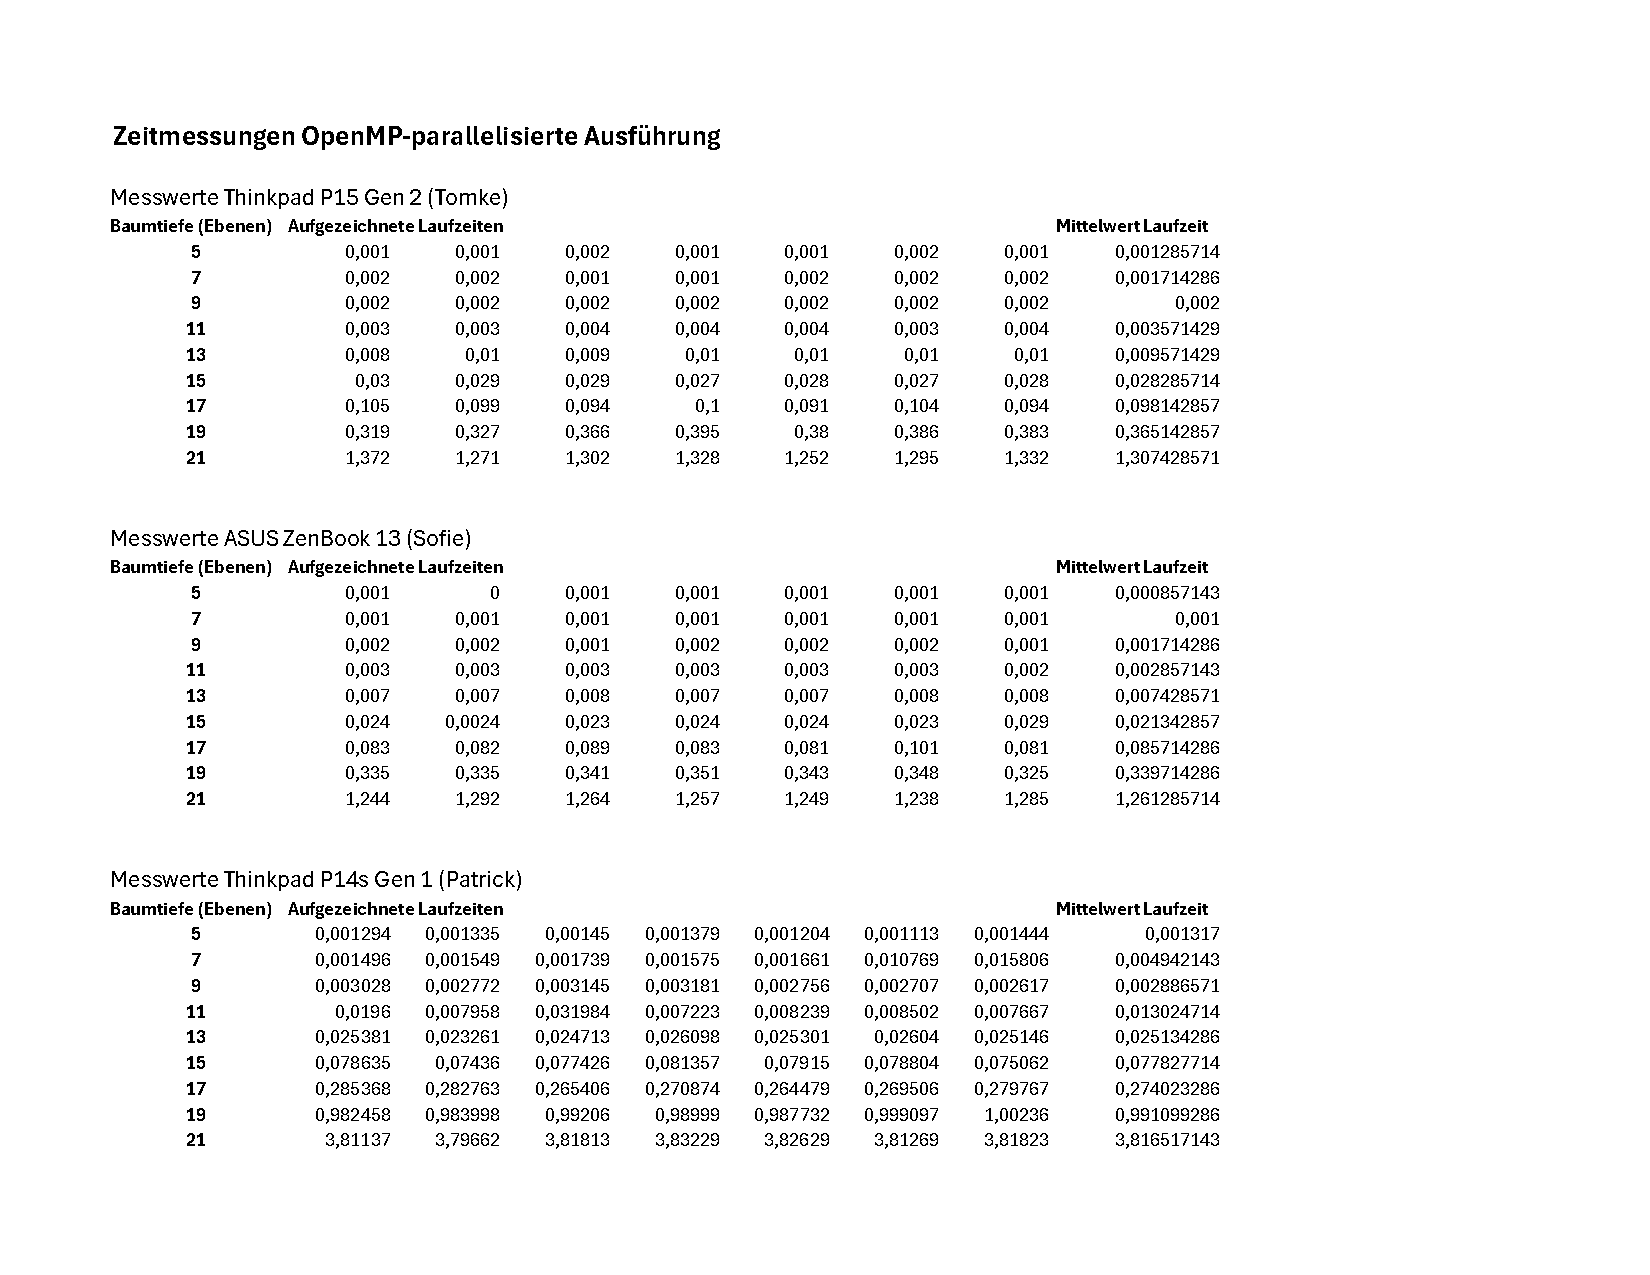
\includepdf[pages=-, fitpaper=true]{appendix/Zeiten_parallel_omp.pdf}
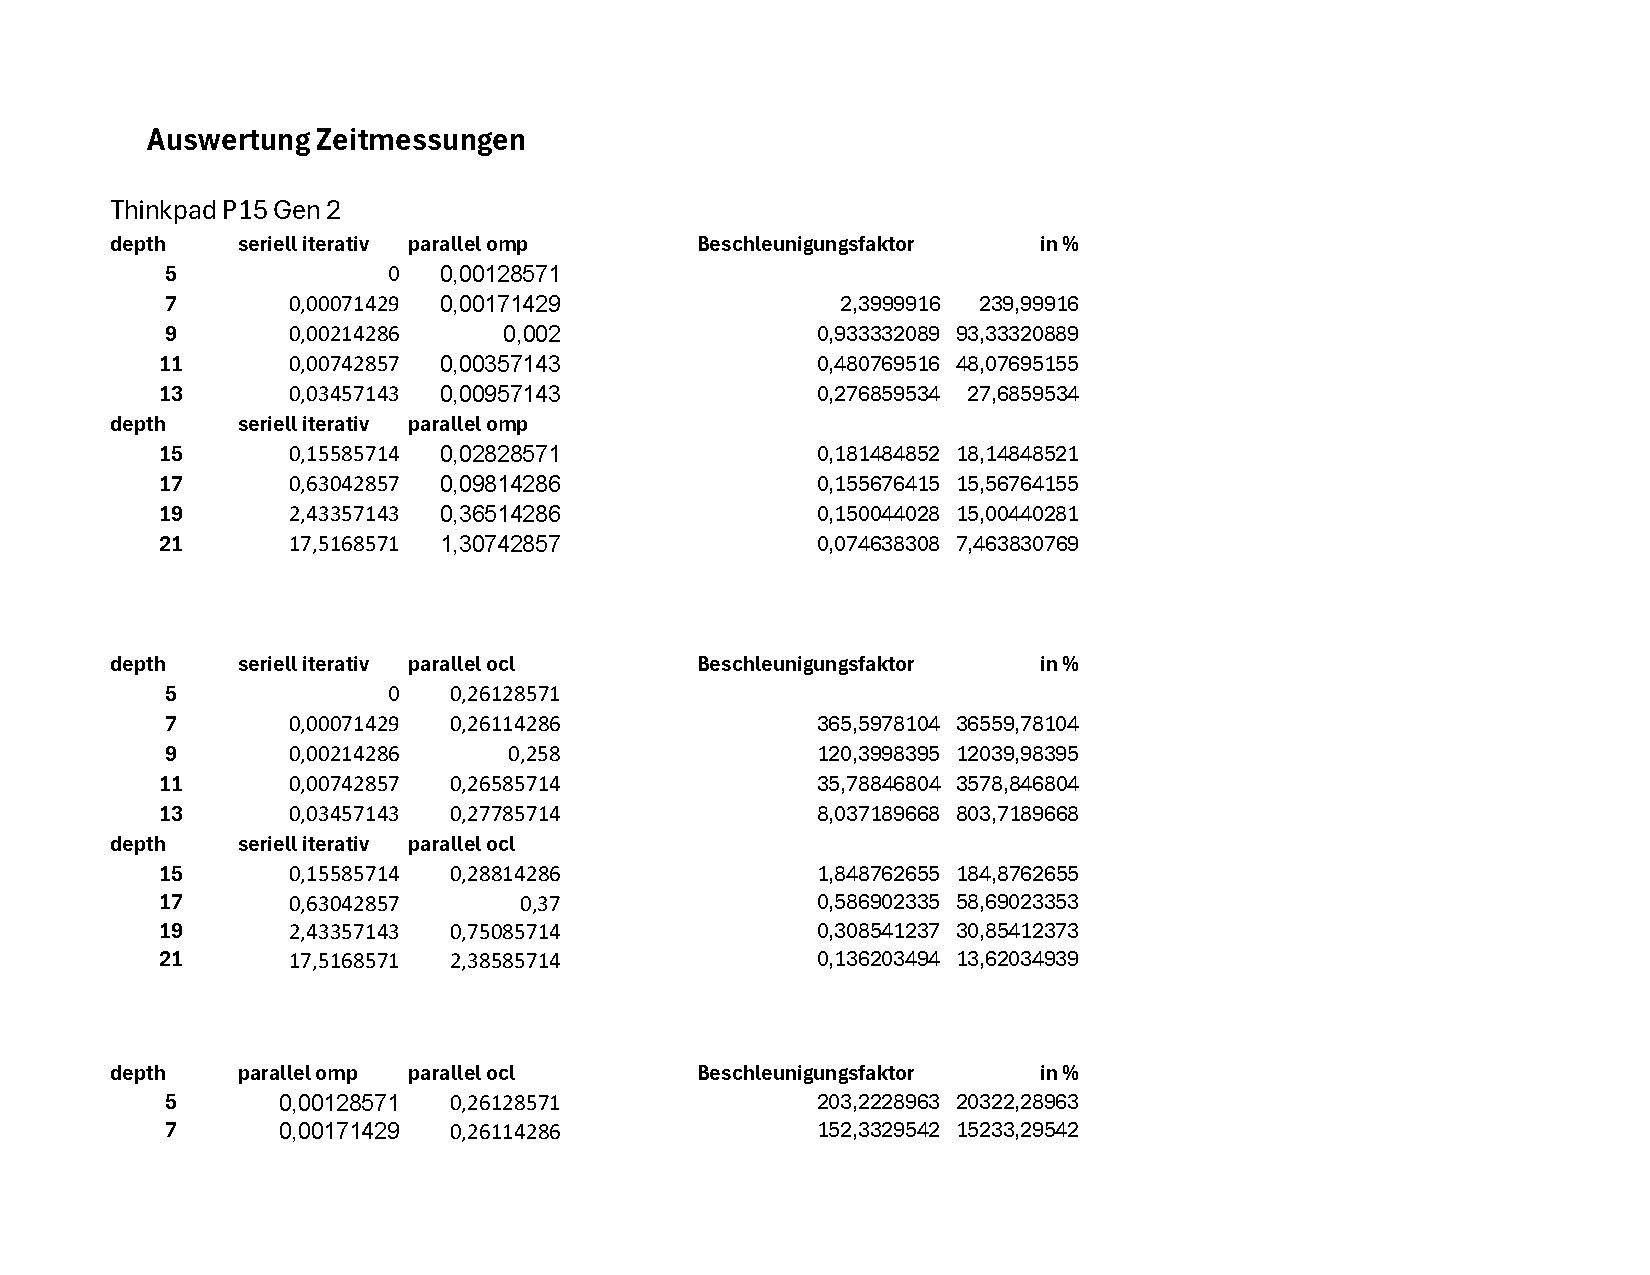
\includepdf[pages=-, fitpaper=true]{appendix/Auswertung_Zeitmessung.pdf}
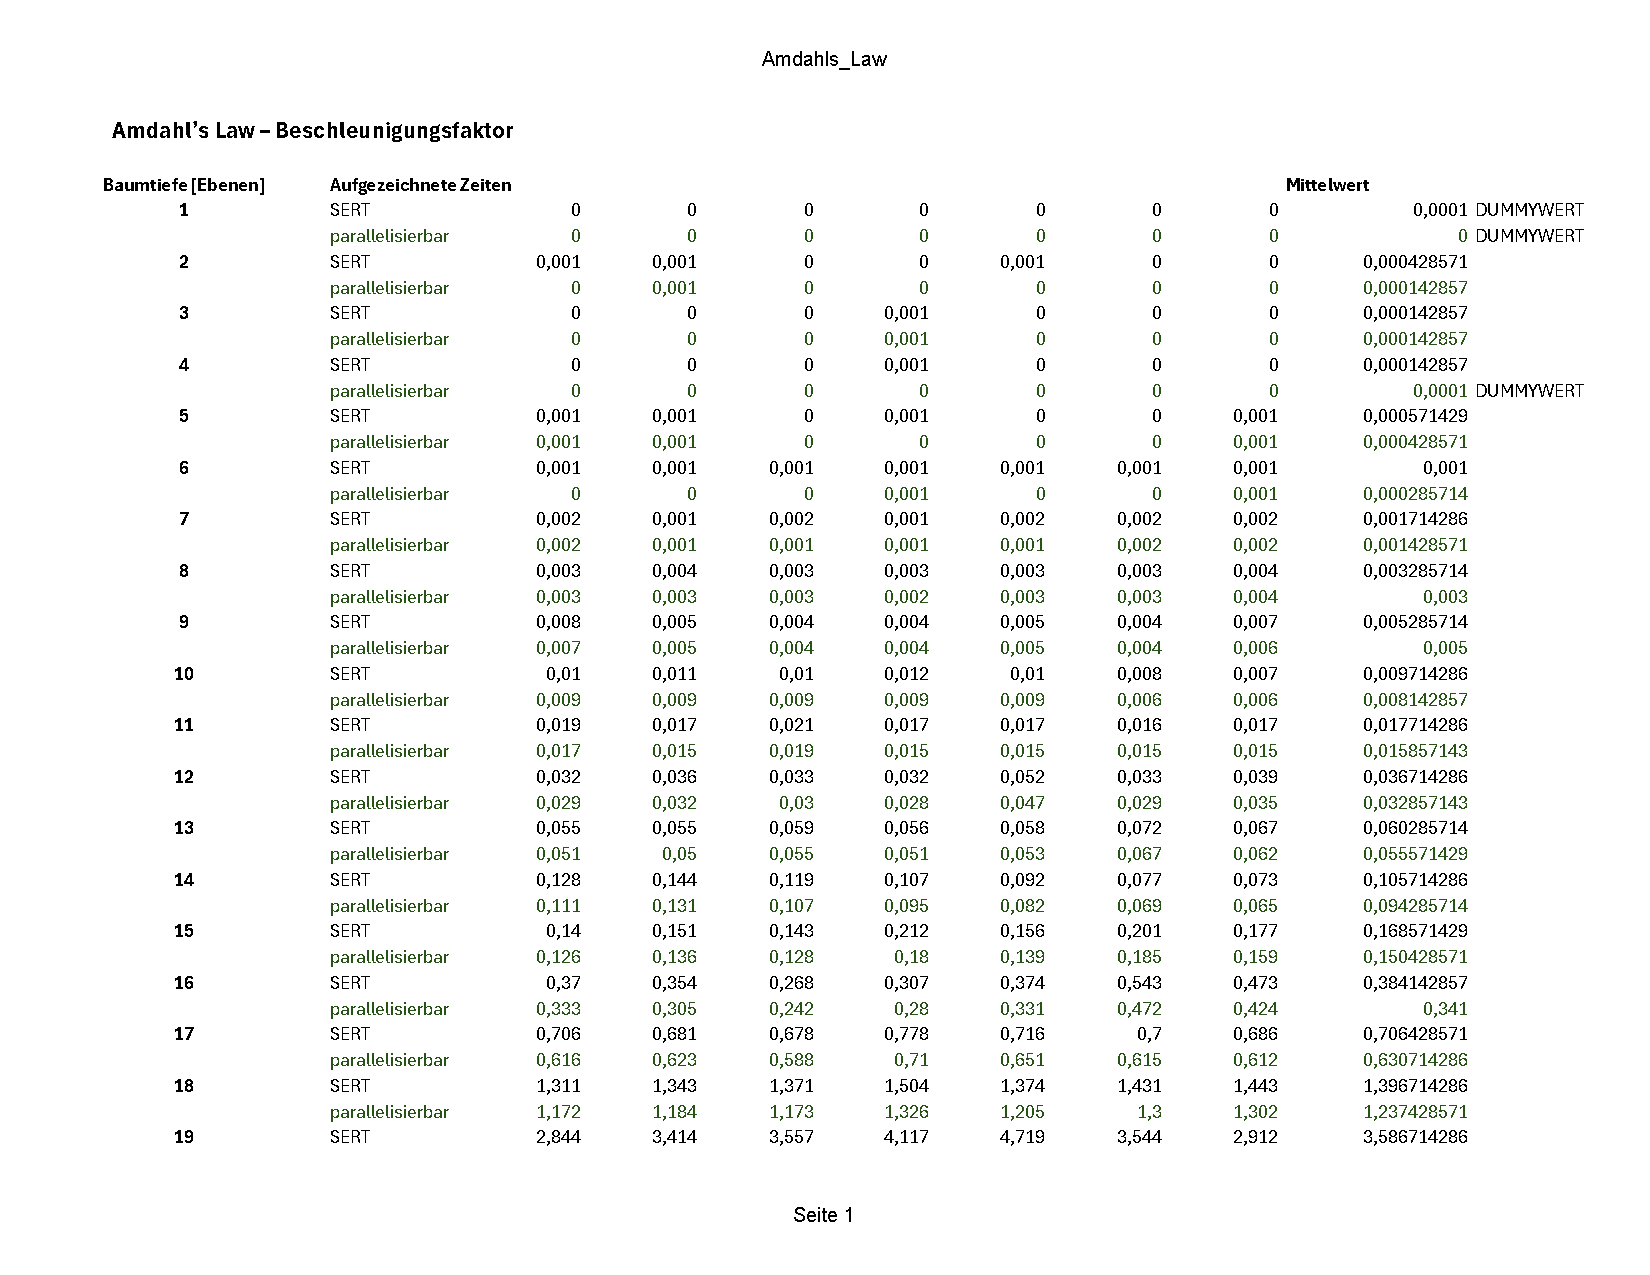
\includepdf[pages=-, fitpaper=true]{appendix/Amdahls_Law.pdf}
\end{document}  